% arara: pdflatex: { synctex: true, shell: true}   
% arara: bibtex
% arara: pdflatex: { synctex: true, shell: true}

%
% uaThesis example (for a thesis written in Portuguese)
%
% the complete list of options and commands can be found in uaThesis.sty
%
%

\documentclass[11pt,twoside,a4paper]{report}
\usepackage[DETI,newLogo]{uaThesis}

\def\ThesisYear{2018}

% optional packages
\usepackage[UKenglish]{babel}
\usepackage{hyperref}
\usepackage{epsfig}     
\usepackage{subfig} 
\usepackage{amsmath}
\usepackage{amssymb}
\usepackage{listings}
\usepackage{color}
\usepackage{fancyvrb}
\usepackage{ifthen}
\usepackage{texments}
\usepackage{fancyhdr}
\usepackage{xspace}% used by \sigla


\definecolor{mygreen}{rgb}{0,0.6,0}
\definecolor{mygray}{rgb}{0.5,0.5,0.5}
\definecolor{mymauve}{rgb}{0.58,0,0.82}


\lstset{ %
	backgroundcolor=\color{white},   % choose the background color; you must add \usepackage{color} or \usepackage{xcolor}; should come as last argument
	basicstyle=\fontfamily{sbc}\selectfont,        % the size of the fonts that are used for the code
	breakatwhitespace=false,         % sets if automatic breaks should only happen at whitespace
	breaklines=true,                 % sets automatic line breaking
	captionpos=b,                    % sets the caption-position to bottom
	commentstyle=\color{mygreen},    % comment style
	deletekeywords={...},            % if you want to delete keywords from the given language
	escapeinside={\%*}{*)},          % if you want to add LaTeX within your code
	extendedchars=true,              % lets you use non-ASCII characters; for 8-bits encodings only, does not work with UTF-8
	%frame=single,	                   % adds a frame around the code
	keepspaces=true,                 % keeps spaces in text, useful for keeping indentation of code (possibly needs columns=flexible)
	keywordstyle=\color{blue},       % keyword style
	%  language=XML,                 % the language of the code
	morekeywords={*,...},            % if you want to add more keywords to the set
	numbers=left,                    % where to put the line-numbers; possible values are (none, left, right)
	numbersep=5pt,                   % how far the line-numbers are from the code
	numberstyle=\tiny\color{mygray}, % the style that is used for the line-numbers
	rulecolor=\color{black},         % if not set, the frame-color may be changed on line-breaks within not-black text (e.g. comments (green here))
	showspaces=false,                % show spaces everywhere adding particular underscores; it overrides 'showstringspaces'
	showstringspaces=false,          % underline spaces within strings only
	showtabs=false,                  % show tabs within strings adding particular underscores
	stepnumber=1,                    % the step between two line-numbers. If it's 1, each line will be numbered
	stringstyle=\color{mymauve},     % string literal style
	tabsize=2,	                   % sets default tabsize to 2 spaces
}

\lstdefinestyle{xml}{
	belowcaptionskip=1\baselineskip,
	breaklines=true,
	%  frame=L,
	%  xleftmargin=\parindent,
	language=XML,
	showstringspaces=false,
	basicstyle=\footnotesize\ttfamily,
	keywordstyle=\bfseries\color{green!40!black},
	commentstyle=\itshape\color{purple!40!black},
	identifierstyle=\color{blue},
	stringstyle=\color{orange},
}

\definecolor{maroon}{rgb}{0.5,0,0}
\definecolor{darkgreen}{rgb}{0,0.5,0}
\lstdefinelanguage{XML}
{
	basicstyle=\ttfamily,
	morestring=[s]{"}{"},
	morecomment=[s]{?}{?},
	morecomment=[s]{!--}{--},
	commentstyle=\color{darkgreen},
	moredelim=[s][\color{black}]{>}{<},
	moredelim=[s][\color{red}]{\ }{=},
	stringstyle=\color{blue},
	identifierstyle=\color{maroon}
}

\usepackage[acronym,automake]{glossaries}
\makeglossaries
\glstoctrue

\newacronym{ad}{AD}{Autonomous Driving}
\newacronym{adas}{ADAS}{Advanced Driver Assistance Systems}
\newacronym{ros}{ROS}{Robot Operating System}
\newacronym{gui}{GUI}{Graphical User Interface}
\newacronym{pcl}{PCL}{Point Cloud Library}
\newacronym{opencv}{OpenCV}{Open Source Computer Vision Library}

% optional (comment to use default)s
%   depth of the table of contents
%     1 ... chapther and sections
%     2 ... chapters, sections, and subsections
%     3 ... chapters, sections, subsections, and subsubsections
\setcounter{tocdepth}{3}

% optional (comment to used default)
%   horizontal line to separate floats (figures and tables) from text
\def\topfigrule{\kern 7.8pt \hrule width\textwidth\kern -8.2pt\relax}
\def\dblfigrule{\kern 7.8pt \hrule width\textwidth\kern -8.2pt\relax}
\def\botfigrule{\kern -7.8pt \hrule width\textwidth\kern 8.2pt\relax}

% custom macros (could also be defined using \newcommand)
\def\I{\mathtt{i}}         % one possible way to represent $\sqrt{-1}$
\def\Exp#1{e^{2\pi\I #1}}  % argument inside braces, i.e., "{}"
\def\EXP#1.{e^{2\pi\I #1}} % argument finishes when a full stop is encountered, i.e., "."
\def\sigla{\LaTeX\xspace}  % use as "blabla \sigla blabla (no need to do "blabla \sigla\ blabla"

\def\AddVMargin#1{\setbox0=\hbox{#1}%
                  \dimen0=\ht0\advance\dimen0 by 2pt\ht0=\dimen0%
                  \dimen0=\dp0\advance\dimen0 by 2pt\dp0=\dimen0%
                  \box0}   % add extra vertical space above and below the argument (#1)
\def\Header#1#2{\setbox1=\hbox{#1}\setbox2=\hbox{#2}%
           \ifdim\wd1>\wd2\dimen0=\wd1\else\dimen0=\wd2\fi%
           \AddVMargin{\parbox{\dimen0}{\centering #1\\#2}}} % put #1 on top #2



\begin{document}

%
% Cover page (use only one of the first two \TitlePage)
%

% First alternative, with a figure
\TitlePage
  %\GRID  % for debugging ONLY
  \HEADER{\BAR\FIG{
\includegraphics[height=60mm]{uaLogoOld}}} % the \FIG{} is optional
         {\ThesisYear}
  \TITLE{Nuno Miguel \newline Soares Silva}
        {Perce\c c\~ao Aumentada para o AtlasCar \newline Augmented Perception for AtlasCar}
\EndTitlePage
\titlepage\ \endtitlepage % empty page

%
% Initial thesis pages
%

\TitlePage
  \HEADER{}{\ThesisYear}
  \TITLE{Nuno Miguel \newline Soares Silva}
        {Perce\c c\~ao Aumentada para o AtlasCar \newline Augmented Perception for AtlasCar}
  \vspace*{15mm}
  \TEXT{}
       {Disserta\c c\~ao apresentada \`a Universidade de Aveiro para cumprimento dos requesitos
        necess\'arios \`a obten\c c\~ao do grau de Mestre em Engenharia de Computadores e Telem\'atica , realizada sob a orienta\c c\~ao
        cient\'\i fica de Paulo Miguel de Jesus Dias, Professor Auxiliar do Departamento de Electr\'onica, Telecomunica\c c\~oes e Inform\'atica da Universidade de Aveiro, de Vitor Manuel Ferreira dos Santos, Professor Associado do Departamento de Engenharia Mec\^ anica e de Miguel Armando Riem de Oliveira, Professor Auxiliar do Departamento de Engenharia Mec\^ anica.}
\EndTitlePage
\titlepage\ \endtitlepage % empty page

\TitlePage
  \vspace*{55mm}
  \TEXT{\textbf{o j\'uri~/~the jury\newline}}
       {}
  \TEXT{presidente~/~president}
       {\textbf{Prof. Doutor A}\newline {\small
        Professor Catedr\'atico da Universidade de Aveiro (por delega\c c\~ao da Reitora da
        Universidade de Aveiro)}}
  \vspace*{5mm}
  \TEXT{vogais~/~examiners committee}
       {\textbf{Prof. Doutor B}\newline {\small
        Professor Catedr\'atico da Universidade de Aveiro (orientador)}}
  \vspace*{5mm}
  \TEXT{}
       {\textbf{Prof. Doutor C}\newline {\small
        Professor associado da Universidade J (co-orientador)}}
\EndTitlePage
\titlepage\ \endtitlepage % empty page

\TitlePage
  \vspace*{55mm}
  \TEXT{\textbf{agradecimentos~/\newline acknowledgements}}
       {\'E com muito gosto que aproveito esta oportunidade para agradecer a todos os que me
        ajudaram durante este longos e penosos anos, cheios de altos e baixos (mais baixos que
        altos)\ldots}
  \TEXT{}
       {Desejo tamb\'em pedir desculpa a todos que tiveram de suportar o meu desinteresse pelas
        tarefas mundanas do dia-a-dia, \ldots}
\EndTitlePage
\titlepage\ \endtitlepage % empty page

\TitlePage
  \vspace*{55mm}
  \TEXT{\textbf{Palavras-chave}}
  {Navega{\c c}\~ao aut\'onoma; ATLASCAR; Agrupamento de dados; Calibra{\c c}\~ao; Etiqueta\c c\~ao de dados; Dete\c c\~ao de Objetos; ADAS.}
  \vspace*{5mm}
  \TEXT{\textbf{Resumo}}
       {Este trabalho baseia-se no desenvolvimento de um pacote ROS para o ATLASCAR 2. O ATLASCAR 2 consiste em um Mitsubishi i-MiEV usado exclusivamente para investiga\c c\~ao de sistemas avan\c cados de assist\^encia \`a condu\c c\~ao no Departamento de Engenharia Mec\^anica da Universidade de Aveiro. O ATLASCAR 2 est\'a equipado com uma c\^amera PointGrey que foi usada para aquisi\c c\~ao de imagens, dois scanners planares LIDAR e um laser de quatro feixes frontais. Este pacote ROS implementa n\'os para dete\c c\~ao semi-autom\'atica de objetos. Estes n\'os s\~ao ut\'eis para etiquetar os dados ligados aos objetos detetados. Estes objetos, na pr\'atica, ser\~ao por exemplo ve\'iculos e pe\~oes na estrada. A manipula\c c\~ao dos dados na imagem foi realizada atrav\'es das bibliotecas de OpenCV. Em paralelo, foi desenvolvido e melhorado a dete\c c\~ao da bola para o pacote de calibra\c c\~ao multi-sensorial.
       	}
\EndTitlePage
\titlepage\ \endtitlepage % empty page

\TitlePage
  \vspace*{55mm}
  \TEXT{\textbf{Keywords}}
  {Autonomous driving; ATLASCAR; Data Clustering; ; Calibration; Data Labelling; Object Detection; ADAS.}
  \vspace*{5mm}
  \TEXT{\textbf{Abstract}}
       {This thesis is based on the development of a ROS package for the ATLASCAR 2. The ATLASCAR 2 consists in a Mitsubishi i-MiEV used exclusively for research of Advanced driver assistance systems (or ADAS) in the Mechanical Engineering Department at University of Aveiro. The ALTASCAR 2 is equipped with a PointGrey camera used to acquire images, two planar LIDAR scanners and a four-beam frontal scanner. This ROS package implements nodes for semi-automatic object detection. This nodes are useful to label data to the detected objects. This objects, in practice, are for example vehicles or pedestrians on the street. The handling of the image data was done through OpenCV libraries. In parallel, it was developed and improved the ball detection for the multi-sensorial calibration package.
       	}
\EndTitlePage
\titlepage\ \endtitlepage % empty page


%
% Tables of contents, of figures, ...
%

\pagenumbering{roman}
\tableofcontents

\cleardoublepage
\listoffigures

\cleardoublepage
\listoftables

\printglossary[type=\acronymtype, title=Acronyms]


% The chapters (usually written using the isolatin font encoding ...)

\cleardoublepage
\pagenumbering{arabic}


% ----------------------------------------------------------------
% Definicao de headers e footers
% ----------------------------------------------------------------
\pagestyle{fancy}
\renewcommand{\chaptermark}[1]{\markboth{\thechapter.#1}{}} % Capítulos em minúsculas
\fancyhf{}                                                  % Reset aos headers e footers
\fancyhead[LE,RO]{\thepage}                               % Header Left-Even (LE), Right-Odd (RO)
\fancyhead[LO]{\leftmark}                                 % Header Left-Odd (LO)
\fancyhead[RE]{\leftmark}                                 % Header Right-Even (RE)
\fancyfoot[LE]{Nuno Miguel Soares Silva}                               % Footer Left-Even (LE)
\fancyfoot[LO]{Nuno Miguel Soares Silva}                               % Footer Left-Odd (LO)
\fancyfoot[RE]{\textit{Master's thesis }}     % Footer Right-Even (RE)
\fancyfoot[RO]{\textit{Master's thesis }}     % Footer Right-Odd (RO)
\renewcommand{\headrulewidth}{0.25pt}                     % Espessura da linha de header
\renewcommand{\footrulewidth}{0.25pt}                     % Espessura da linha de footer
\addtolength{\headheight}{0.5pt}                          % Espaçamento para a linha

\chapter{Introduction}
Technological studies in the fields of \gls{adas} and \gls{ad} have been growing in the past decades in the automobile industry and in the academic environment. 

It is important in \gls{ad} and \gls{adas} to implement machine learning methods so that the vehicles recognize what objects are in their surroundings. Therefore, labelled data is necessary to train machine learning algorithms. Data labelling is the solution to create datasets that will serve as input to learning algorithms.

This thesis is focused on the research of methods to register data into labels using a camera and \gls{lidar} sensors in ATLASCAR 2, so that the vehicle can later create a model of the objects it will detect and follow.

This dissertation will also improve some previous work, namely the calibration process in ATLASCAR 2. In addition to the calibration, a tool for image labeling and tracking of objects will be developed. This tool will be used to gather image templates while tracking objects in the camera video. 

\section{ATLAS Project}

ATLAS is a project developed by the Group of Automation and Robotics at the Department of Mechanical Engineering of the University of Aveiro, Portugal. The mission of the ATLAS project is to develop and enable the proliferation of advanced sensing and active systems designed for implementation in automobiles and affine platforms. Advanced active systems being improved, or newly developed, use data from vision, laser and other sensors. 

The ATLAS project has vast experience with autonomous navigation in controlled environments and is now evolving to deal with real road scenarios. To ensure that the developments are meeting the ATLAS project mission statement, a full sized prototype, the ATLASCAR 1, has been equipped with several state of the art sensors (\cite{LARlabs}). Currently, ATLASCAR 2 is the new full sized prototype being used for research equipped with \gls{lidar} sensors and a camera.

The ATLAS Project was created in 2003 and began with robots developed to participate at \gls{ad} competitions taking place at Portuguese National Robotics Festival. From this project, three small-sized platform robots were built (figure \ref{fig:atlasproto}). These robots were very successful having won prizes in some of the robotics competitions. 


\begin{figure}[htp]
	
	\centering
	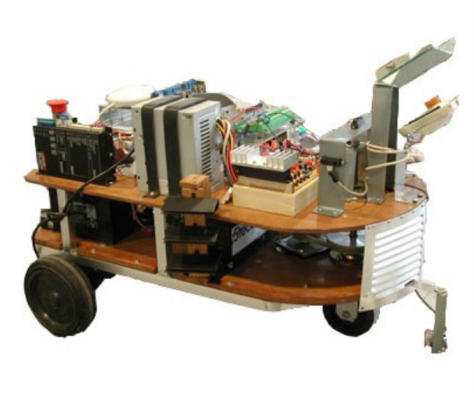
\includegraphics[width=.3\textwidth]{capintro/imgs/atlas1}\hfill
	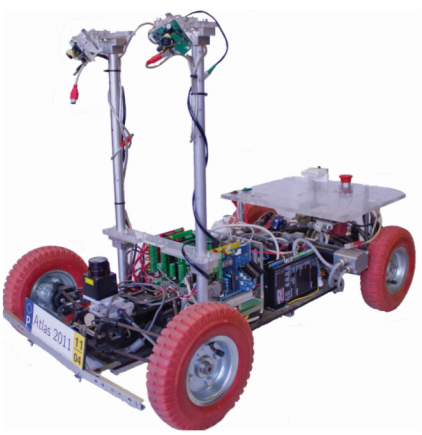
\includegraphics[width=.3\textwidth]{capintro/imgs/atlas2000}\hfill
	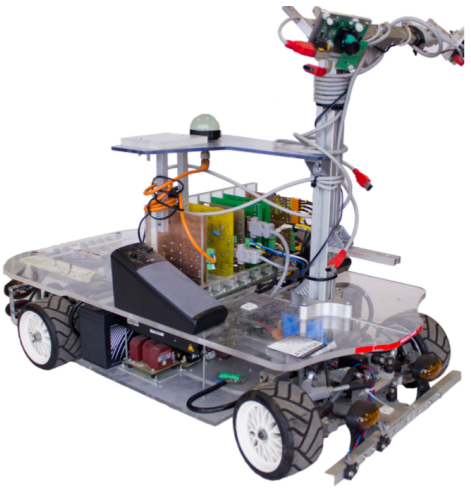
\includegraphics[width=.3\textwidth]{capintro/imgs/atlasmv}
	
	\caption{ATLAS project small-sized prototypes \cite{LARlabs}}
	\label{fig:atlasproto}
	
\end{figure}

As the project grew, it evolved into full-sized prototypes: the ATLASCARs. ATLASCAR1 (figure \ref{fig:atlascar1}) is the first full-sized platform and it is based on a Ford Escort Station Wagon. The ATLASCAR1 was equipped with several \gls{lidar} sensors and cameras. Data about its environment is gathered by the scanners which is then processed building perception into the car allowing the car to actuate and move autonomously. 

\begin{figure}[htp]
	
	\centering
	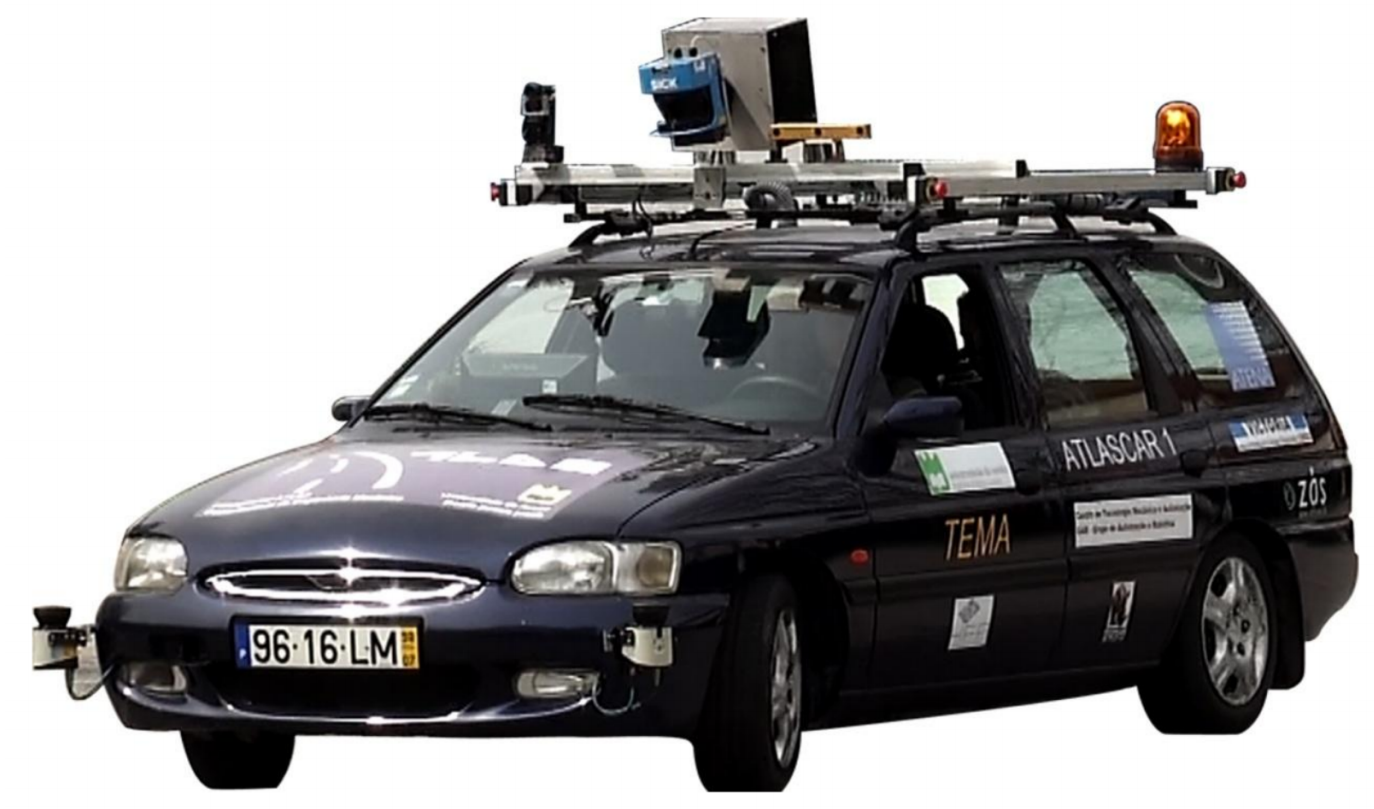
\includegraphics[width=0.9\textwidth]{capintro/imgs/atlascar1}
	
	\caption{ATLASCAR1 based on the Ford Escort platform \cite{LARlabs}}
	\label{fig:atlascar1}
	
\end{figure}

The ATLASCAR1 brought successful results. In the end, the vehicle was able to move and execute maneuvers autonomously in small and controlled places. The ATLASCAR1 was then replaced by a more recent vehicle. The ATLASCAR2 (figure \ref{fig:atlascar2}) is the new full-sized platform of the ATLAS project and it is based on a Mitsubishi i-MiEV. This is the vehicle used for research in this dissertation. The ATLASCAR2 is equipped with various \gls{lidar} sensors and a camera. It is also a full electric vehicle which will be easier to modify, test and control. 

\begin{figure}[htp]
	
	\centering
	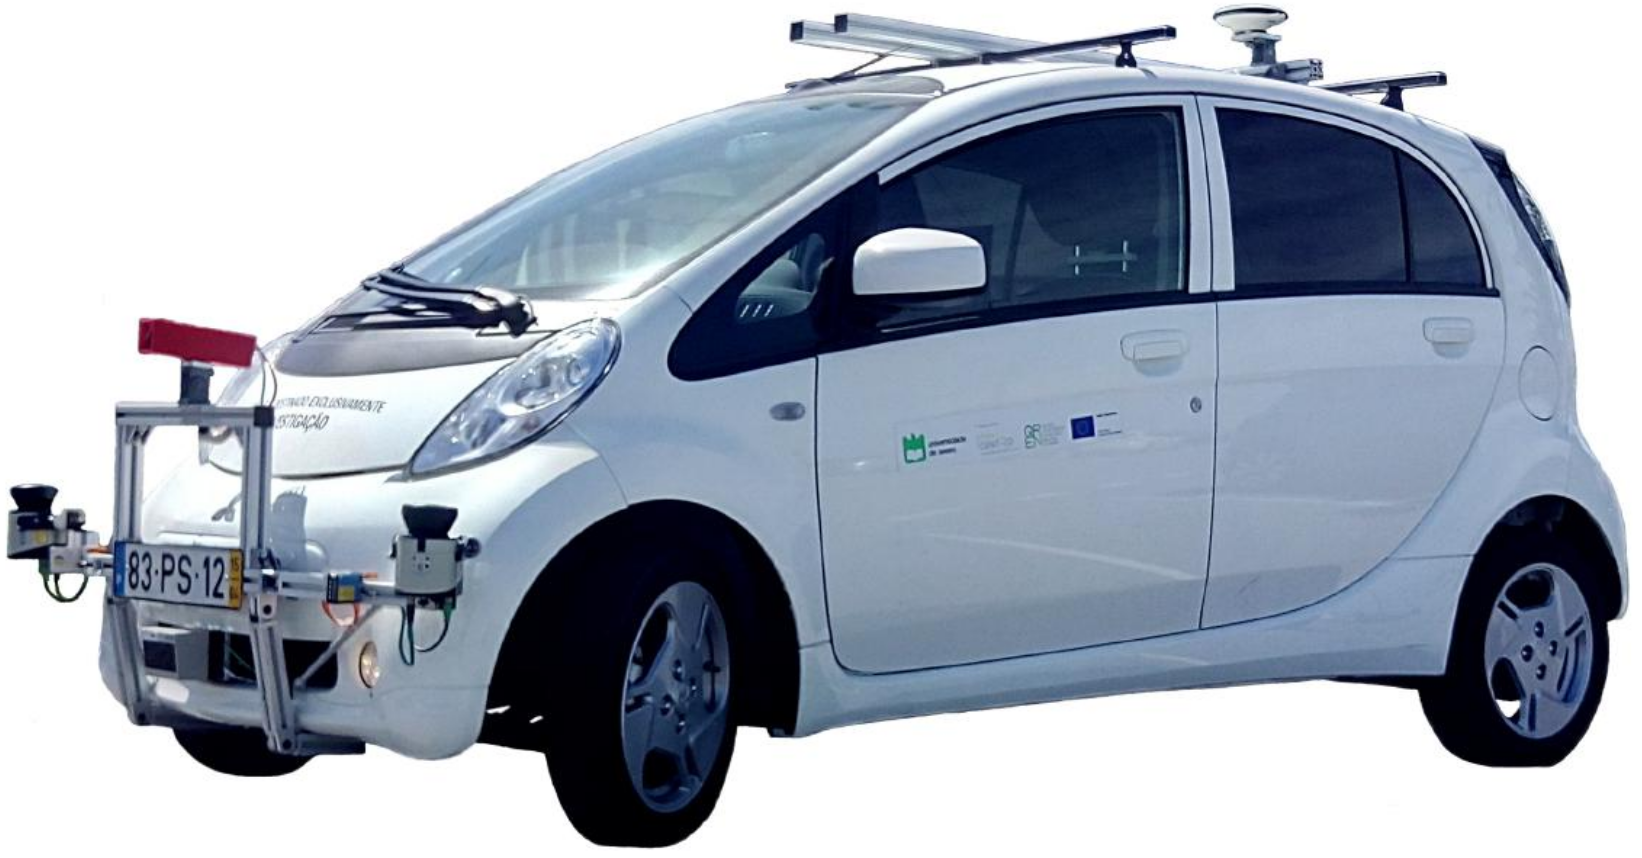
\includegraphics[width=0.9\textwidth]{capintro/imgs/atlas2.png}
	
	\caption{ATLASCAR 2 based on the Mitsubishi i-MiEV platform \cite{LARlabs}}
	\label{fig:atlascar2}
	
\end{figure}


\section{Motivation}

\gls{ad} and \gls{adas} often make use of machine learning. Deep learning algorithms utilize neural and convolutional networks for images and range-based sensor data. In the fields of machine learning, images are often used as input templates to create object models. In an image sequence it is possible to track an object and obtain samples of the target's location. This way it is possible for an algorithm to automatically recognize an object.

While registering the position of the objects in an image sequence, it is important to tell what those objects are. Labelling is the act to classify objects in a certain group. As the annotation is done, when selecting an object, the user should enter a label that identifies the target making it easy for the learning algorithm to recognize to object afterwards.

The objective and importance of tagging samples of images with a label is to assign metadata in the form of a keyword to later allow an application to retrieve this information and easily construct a database. However, most labelling for images is currently done with non optimized manual procedures.

In the end of this dissertation, the ATLASCAR2 will have a labelling system that fuses images retrieved from the camera with the laser data, creating a semi automatic object tracking system that offers the possibility to retrieve various image template sequences and store metadata about them. This metadata contains, for instance, the label, object related identification markers and position of the object in the image and in the real world relatively to the ATLASCAR2.

\section{Objectives}
The objectives for this dissertation are, firstly, to improve the calibration of the camera, in particular regarding the detection of the ball by the camera in the existing multi-sensor calibration package developed using \gls{ros}. Secondly, the development of another \gls{ros} package used for semi-automatic detection and labelling of objects in the field of view.

The calibration package was already developed by \cite{VieiradaSilva2016}. The methods used to detect the ball in the camera image were basically filtering values from the \gls{hsv} color space. There are methods that can make this detection more robust that will be explained in this thesis. 

The detection, tracking and labelling system will combine the image data and the laser data from the sensors to create a semi-automatic tracking system that allows the user to associate an object category to the target and create datasets with metadata from the labelling.


\section{Document Structure}

This document is composed by seven chapters including the introduction. The second chapter describes the related work previously done on ATLASCAR 2 as well as a literature review detailing the most significant milestones on the history of autonomous driving and a research on image labelling datasets. 

In the third chapter, the experimental structure of this dissertation will be described depicting the hardware (ATLASCAR2 and sensors) and the software (\gls{ros}, \gls{lartk} and \gls{pcl}). 

In the fourth chapter, the implementation of the calibration node will be explained presenting its features, the base algorithm and how the calibration package was modified in order to improve the ball detection. 

In the fifth chapter, the detection, tracking and labelling node development will be explained, firstly by describing how the image tracking is done, then clarifying how to track objects using the \gls{lidar} sensors and finally using both the image and laser sensor data. This chapter also features the created datasets and some extra tools used to aid in the labelling. 

The sixth chapter presents the results of the ball detection and integration with the calibration package will be shown and the outcome of the labelling node will also be analyzed using some datasets produced by the same. 

The final chapter the conclusions of this thesis are presented and some future work related to the scope of this dissertation is proposed.


\chapter{State of the art}

\section{Milestones on the history of autonomous vehicles}

Overall, motorized road transport led to the accidental deaths of around 200,000 US citizens in the 1920s; by far the greatest number of these were pedestrians. \cite{Kroger2016} The idea of substituting error-prone humans with technology thus practically suggested itself. The first registered experiments for \gls{ad} have been conducted circa the 1920's  \cite{TheMilwaukeeSentinel} in Milwaukee. A 1926 Chandler was equipped with a transmitting antennae and was radio-controlled by a second car that followed it.

\begin{figure}[htp]
	
	\centering
	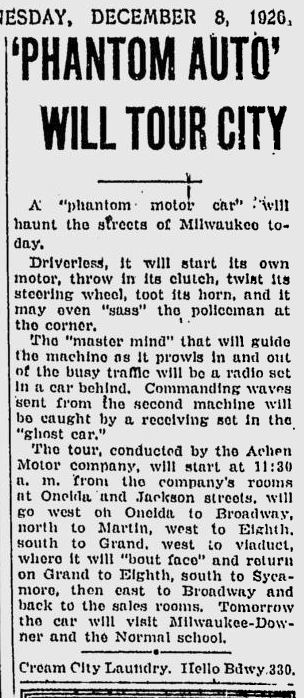
\includegraphics[width=0.25\textwidth]{capstate/imgs/jornal.png}
	
	\caption{The Milwaukee Sentinel - 8 Dez 1926 - 'Phantom Auto' Will Tour City}
	\label{fig:waymo}
	
\end{figure}

In the 1950s promising trials in \gls{ad} took place. General Motors conducted experiments in miniature models along with the electronic manufacturer \gls{rca}. The two companies later developed a full size system that was successfully demonstrated completing a test route of one mile.  \cite{Kroger2016}

In the 1980s, pioneer Ernst Dickmanns designed a vision-guided Mercedes Benz along with the Bundeswehr University Munich engineering team, achieving a speed of 63 km/h on streets with no traffic. In the late 80s, projects with both \gls{lidar} scanners and computer vision were carried out. In 1989 the first experiments with vehicles making use of neural networks were conducted. \cite{Pomerleau1989}

Since then, many companies and research organizations have been developing various prototype cars. In the past decade, electric motored cars have emerged and new opportunities for \gls{ad} and \gls{adas} research have appeared. 

Waymo, the Google self-driving car project, begun testing driverless cars without someone at the driver position. The Waymo project started in 2009 and it counts more than 5 million miles self-driven. Google has recently partnered with Jaguar and designed self-driving Jaguar I-PACEs (figure \ref{fig:waymo}). Tests on the newest self-driving Waymo's vehicle will be conducted in 2018. \cite{Waymo}


\begin{figure}[htp]
	
	\centering
	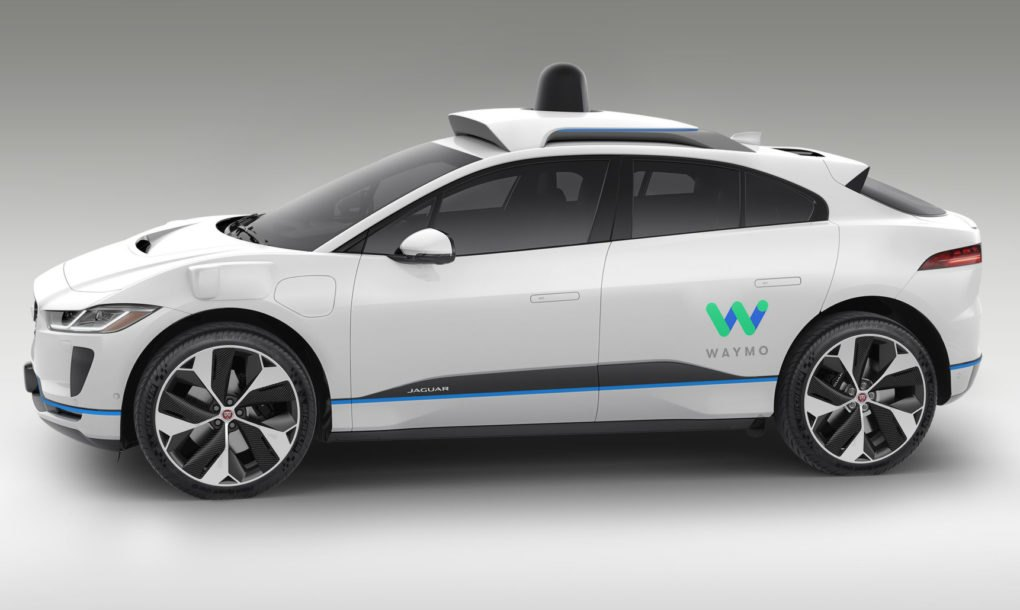
\includegraphics[width=0.9\textwidth]{capstate/imgs/waymo}
	
	\caption{Waymo's Jaguar I-PACE}
	\label{fig:waymo}
	
\end{figure}

Another example of an autonomous vehicle project is the Uber \gls{atc} car based on an hybrid Ford Fusion (figure \ref{fig:uber}). The vehicle is equipped with state of the art \gls{lidar} scanners, and several vision-based sensors and radars.

\begin{figure}[htp]
	
	\centering
	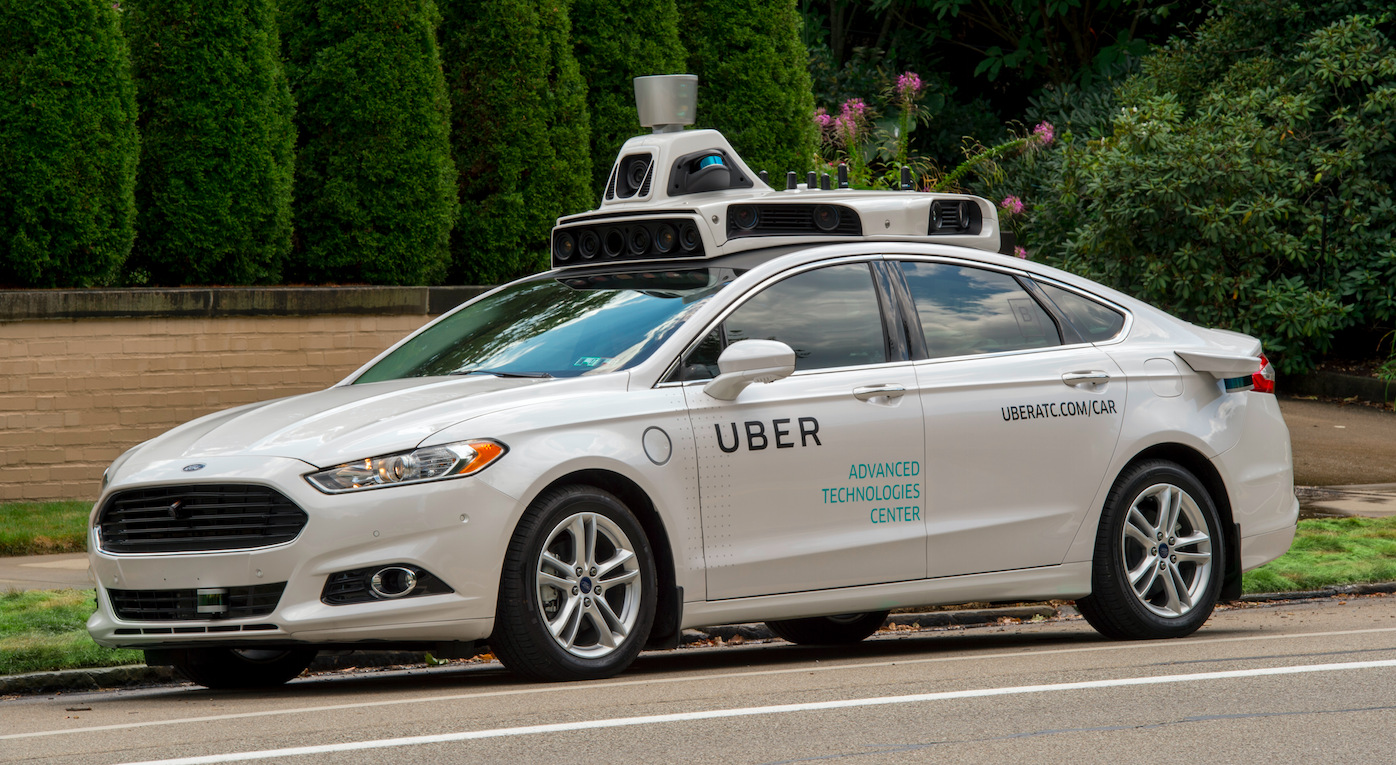
\includegraphics[width=0.9\textwidth]{capstate/imgs/uber}
	
	\caption{Ford Fusion Uber ATC car}
	\label{fig:uber}
	
\end{figure}

Audi released its A8 (figure \ref{fig:audi}) and the company stated that they would be the first manufacturer to use laser scanners in addition to cameras and others sensors in autonomous vehicles. The vehicle was designed to a level 3 autonomous driving: it is capable of self-driving with the expectation that the human driver will respond appropriately to a request to intervene. The Audi AI traffic jam pilot takes over the driving task in slow-moving traffic up to 60 km/h. \cite{AudiMediaCenter}

\begin{figure}[htp]
	
	\centering
	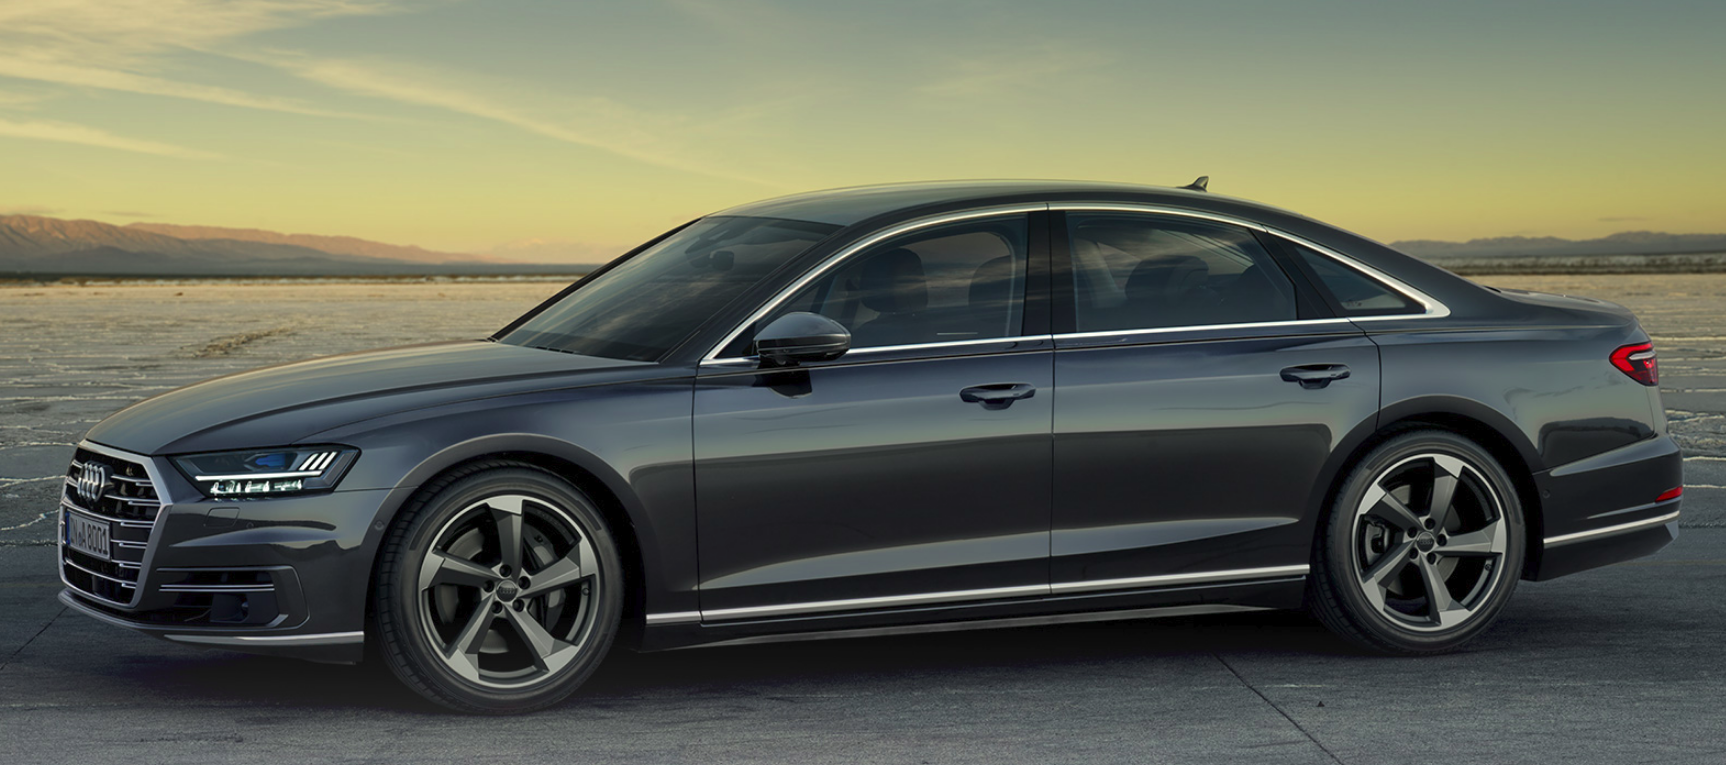
\includegraphics[width=0.9\textwidth]{capstate/imgs/audi}
	
	\caption{The new Audi A8}
	\label{fig:audi}
	
\end{figure}

Like the University of Aveiro, many other universities and research institutes study the \gls{ad} and \gls{adas} paradigms.

Another interesting autonomous vehicle project is the \gls{scot} vehicle (figure \ref{fig:scot}), conducted by the \gls{smart}. \cite{Singapore-MITAllianceforResearchandTechnology} Like the ATLASCAR 2, \gls{scot} is also a Mitsubishi i-MiEV used to research \gls{adas} and \gls{ad} at \gls{smart} and it is designed for operations on public roads. The \gls{scot} vehicle also relies on \gls{lidar} sensors similar to ATLASCAR 2. \cite{Teo}

\begin{figure}[htp]
	
	\centering
	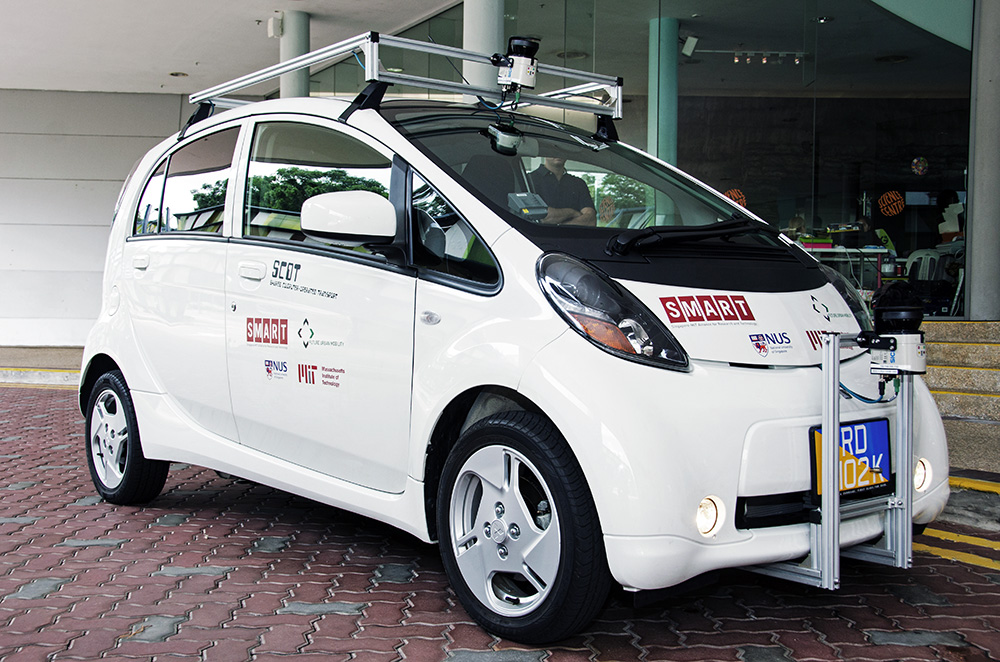
\includegraphics[width=0.9\textwidth]{capstate/imgs/scot}
	
	\caption{SCOT - Shared Computer-Operated Transit vehicle}
	\label{fig:scot}
	
\end{figure}


\section{Multi Sensor Calibration}

For vehicles to become fully autonomous, it is needed for them to recognize their environment. The perception of their surroundings is obtained from data acquired through ranged-based sensors. The more sensors the vehicle has, the more accurate it can be about the environment. A car equipped with several sensors needs to know the position of each sensor so that the readings can be aligned and exact perception can be obtained. 

For this dissertation, the camera calibration is to be improved. Multi sensor calibration in ATLASCAR 2 is done using a ball as a target. While moving the ball around the sensors, a point cloud is created for each sensor. These point clouds are aligned so that the estimate pose of each sensor can be obtained using an arbitrary sensor as reference. \cite{VieiradaSilva2016}

\section{Image Labelling}
Tracking of objects in image processing is done frequently using bounding boxes around the target. These boxes are often linked to a class in which the object in the template represents. Image labelling is the act of relating the object to this class, or more specifically, the label. 

\subsection{KITTI Dataset}
Some image labelling datasets already exist. One of them and probably the most well-known in the fields of \gls{ad} is the \gls{kitti} dataset. \cite{KarlsruheInstituteofTechnology} The \gls{kitti} Dataset was captured from a Volkswagen station wagon (figure \ref{fig:kitticar}) for use in mobile robotics and \gls{ad} research. The \gls{kitti} benchmark suite is born in 2012 at Karlsruhe Institute of Technology by the need to have a dataset to classify objects on the streets. This project has grown by increasingly adding more results with more sensors. The \gls{kitti} benchmark started with the stereo, flow and odometry benchmarks and today it includes standards for object tracking and more. 

\begin{figure}[htp]
	
	\centering
	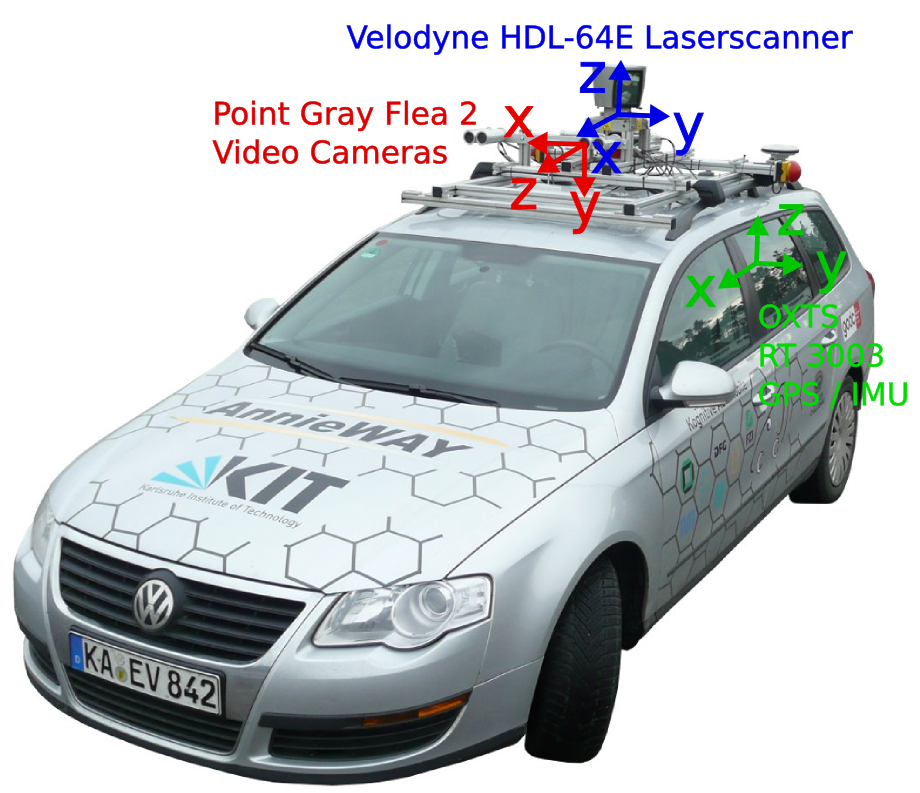
\includegraphics[width=0.7\textwidth]{capstate/imgs/kitticar}
	
	\caption{Volkswagen Station Wagon used in the KITTI Dataset}
	\label{fig:kitticar}
	
\end{figure}

Just like ATLASCAR 2, the car used in the \gls{kitti} dataset is equipped with \gls{lidar} sensors and Point Grey Video Cameras. The dataset is used for automatic recognition and tracking of vehicles and pedestrians. It consists in image sequences (see figure \ref{fig:kittiresult}) and a text file in which, for each frame the various objects in the field of view are depicted with and identification number, a label, and coordinates about their position regarding the car and in the image. \cite{Geiger} 

\begin{figure}
\begin{center}
	\begin{lstlisting}[caption={KITTI dataset file snippet.}, language=c++, label={lst: pop_grid}]
	...
	3 1 Cyclist 0 0 -1.931469 759.786603 146.098339 954.280160 374.000000 1.739063 0.824591 1.785241 1.821119 1.569936 5.783265 -1.642450
	3 2 Pedestrian 0 0 -2.547728 1154.836779 148.360923 1241.000000 321.627088 1.714062 0.767881 0.972283 6.463579 1.474131 7.560739 -1.860031
	4 -1 DontCare -1 -1 -10.000000 252.530000 168.660000 284.460000 202.850000 -1000.000000 -1000.000000 -1000.000000 -10.000000 -1.000000 -1.000000 -1.000000
	4 0 Van 0 0 -1.808333 290.287584 146.641981 444.387179 269.473545 2.000000 1.823255 4.433886 -4.934786 1.601945 14.098646 -2.139796
	4 1 Cyclist 0 0 -1.929519 767.158958 140.942948 961.992360 374.000000 1.739063 0.824591 1.785241 1.881359 1.534695 5.785600 -1.631447
	4 2 Pedestrian 1 0 -2.557045 1180.675035 151.025283 1241.000000 325.015204 1.714062 0.767881 0.972283 6.516488 1.497786 7.267796 -1.846627
	...	\end{lstlisting}
\end{center}
\end{figure}

In listing \ref{lst: pop_grid} it can be analyzed an example snippet in which there are two lines of what the \gls{kitti} dataset looks like. Each line starts with the frame ID and the ID of the object being tracked. Then it is added a label to classify this object. There are also flags to indicate if the object is either truncated or occluded in the image sequence. The following numbers consist in the alpha (observation angle of object), the left, top, right and bottom of the 2D bounding box, the height, width and length of the 3D bounding box and its XYZ coordinates. The last number consists in the 3D rotation angle in the Y axis. \cite{Team} The legend of this \gls{kitti} dataset snipped would be the following:

\begin{center}
	\begin{lstlisting}[caption={KITTI dataset file snippet legend.}, label={lst: kitti_legend}]
	frame_id object_id label truncated occluded alpha left top right bottom height width length x y z rotation_y	\end{lstlisting}
\end{center}

The legend in listing \ref{lst: kitti_legend} is not included in the dataset files. Analyzing the snippet, it is possible to locate a a cyclist and a pedestrian in frame 3 and the same cyclist and pedestrian (because they have the same object\_id) in the next frame with also a van. The \texttt{DontCare} label is often shown representing an object detected that is not related to the scope of the \gls{kitti} dataset. Other information indicate where these objects are found relatively to the car.

\begin{figure}[htp]
	
	\centering
	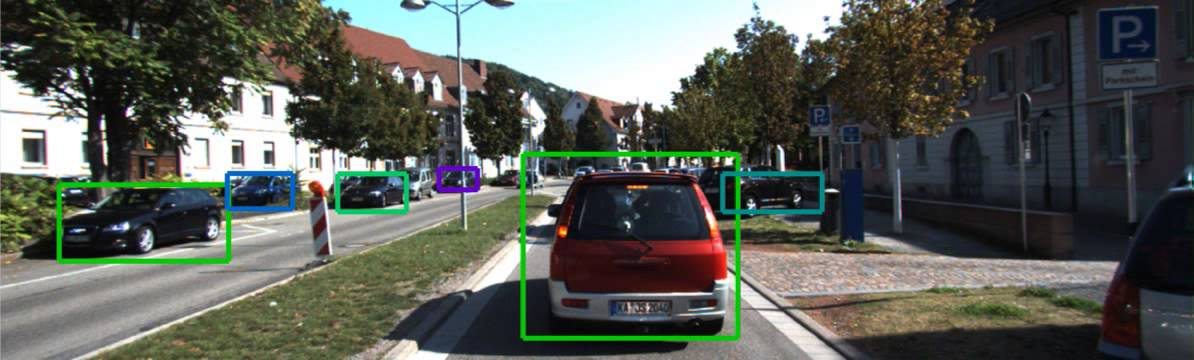
\includegraphics[width=0.99\textwidth]{capstate/imgs/kittiresult}
	
	\caption{Sequence example of tracking by detection using the \gls{kitti} dataset}
	\label{fig:kittiresult}
	
\end{figure}
	
\subsection{HumanEva II Dataset}
The HumanEva II Dataset from the \gls{mpii} was also a dataset worth researching. Although it is used for pedestrian detection only, it was important to have a comparator with the \gls{kitti} dataset, specially regarding its structure. 
This dataset appears in the demand for a way to represent information about detection and tracking of humans and their poses captured by a single image camera. The HumanEva dataset has information about the bounding boxes position used to track and detect pedestrian limb poses. This information is useful to know which direction the person is facing from the 3D skeleton derived from the pose. The data structure in the dataset is similar to a XML file. For each frame in the image sequences there are several bounding boxes with the respective coordinates. \cite{Sigal}

\begin{figure}
\lstinputlisting[label={lst:humaneva_snip}, caption={HumanEva dataset file snippet.},language=xml]{capstate/files/humaneva_snip.xml}
\end{figure}

\begin{figure}[htp]
	
	\centering
	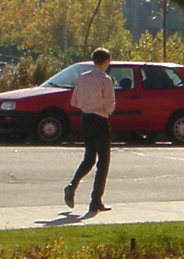
\includegraphics[width=0.5\textwidth]{capstate/imgs/00050.png}
	
	\caption{Example image of the HumanEva dataset that generated the snippet in listing \ref{lst:humaneva_snip} }
	\label{fig:00050}
	
\end{figure}

By looking at listing \ref{lst:humaneva_snip}, in this dataset snippet is easy to identify the interest points in the given frame. The files are a set of annotations called $annotationList$ in which a path to the image corresponding to the frame is given. For each image there is $annorect$ with bounding box coordinates $(x1,y1,x2,y2)$, a score, silhouette, articulation and viewpoint id. There is also a section called $annopoints$ where sets of points with an id are annotated.

\subsection{Other relevant datasets}
Other datasets included in the research for this dissertation are found in \gls{ethz} and in \gls{epfl} projects. 
\subsubsection{ETHZ dataset}
\gls{ethz} conducted studies for detection and tracking of people on the street. The dataset is simple: for each frame there are several bounding boxes in the image.
\begin{figure}
\begin{center}
	\begin{lstlisting}[label={lst:ETHZ}, caption={ETHZ dataset dataset file snippet.},language=c++]
	...
	"left/image_00000015_0.png": (222, 177, 268, 312), (373, 105, 463, 393), (458, 220, 487, 285), (310, 225, 327, 265), (335, 228, 352, 264), (267, 228, 281, 261);
	"left/image_00000016_0.png": (220, 172, 266, 313), (378, 407, 476, 102), (462, 219, 486, 285), (312, 223, 327, 264), (337, 226, 352, 262), (267, 231, 279, 260);
	"left/image_00000017_0.png": (219, 173, 267, 316), (394, 94, 489, 423), (313, 222, 330, 262), (338, 227, 354, 262), (267, 228, 279, 260);
	...	\end{lstlisting}
\end{center}
\end{figure}

\begin{figure}[htp]
	
	\centering
	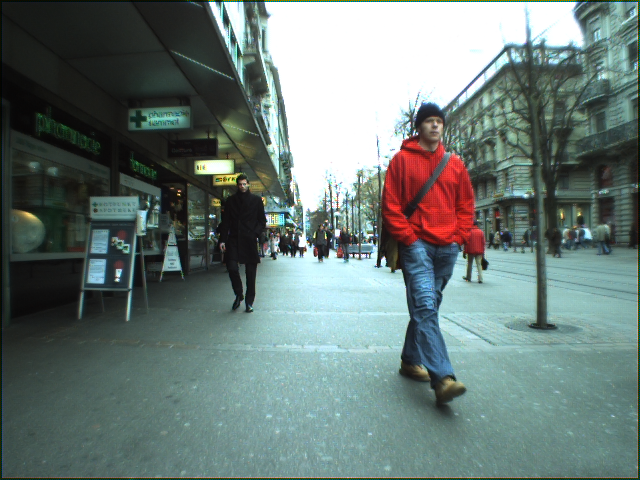
\includegraphics[width=0.7\textwidth]{capstate/imgs/image_00000016_0.png}
	
	\caption{One of the images of the \gls{ethz} dataset that generated part of the snippet in listing \ref{lst:ETHZ} }
	\label{fig:ETHZ}
	
\end{figure}

This dataset is focused just in the detection and tracking of pedestrians in the image. \cite{ETHZEidgenossischeTechnischeHochschuleZurich} In listing \ref{lst:ETHZ} each line is composed with a string defining a path to the image representing the actual frame, followed by tuples of four elements $(x1,y1,x2,y2)$ representing the bounding boxes where pedestrians are found in the respective frame. 

\subsubsection{EPFL dataset}
The \gls{epfl} designed a dataset for multiple people in a camera environment, independent of the scenario. This dataset used various synced video cameras filming the same area in different angles. 

\begin{figure}
\begin{center}
	\begin{lstlisting}[label={lst:basket}, caption={ETHZ dataset file snippet.},language=c++]
									...
									1 80 45 99 98 9363 0 0 1 "PERSON"
									1 80 45 99 98 9364 0 0 0 "PERSON"
									1 77 45 96 98 9365 0 0 1 "PERSON"
									1 74 45 93 98 9366 0 0 1 "PERSON"
									1 71 46 90 99 9367 0 0 0 "PERSON"
									2 81 45 110 126 0 0 0 0 "PERSON"
									2 80 45 109 126 1 0 0 1 "PERSON"
									2 80 45 109 126 2 0 0 1 "PERSON"
									2 80 45 109 126 3 0 0 1 "PERSON"
									2 80 45 109 126 4 0 0 1 "PERSON"
									...	\end{lstlisting}
\end{center}
\end{figure}

\begin{figure}[htp]
	
	\centering
	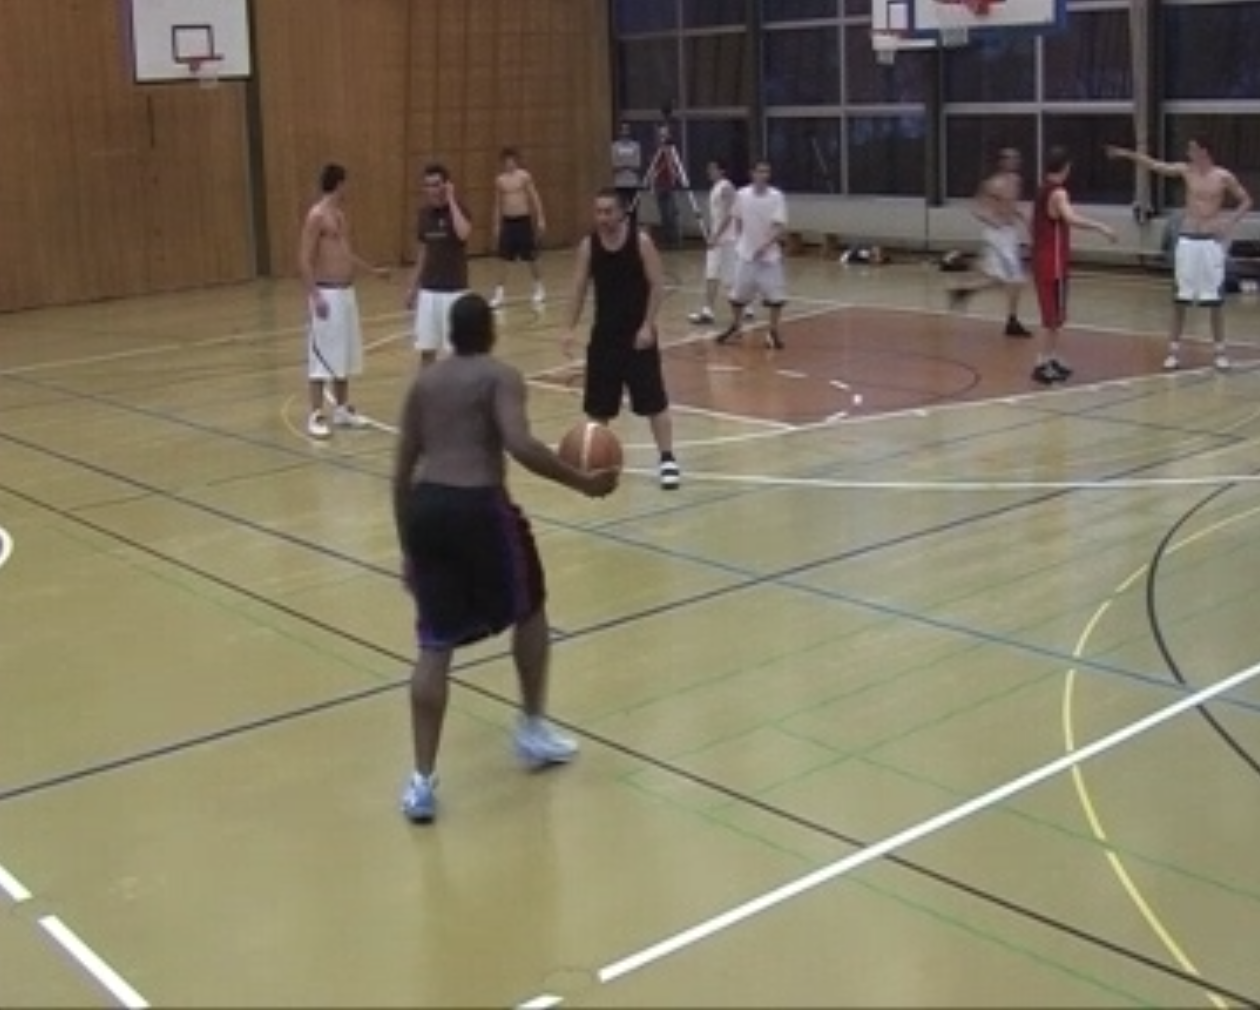
\includegraphics[width=0.7\textwidth]{capstate/imgs/basket.png}
	
	\caption{One of the images of the \gls{epfl} dataset that generated part of the snippet in listing \ref{lst:basket} }
	\label{fig:basket}
	
\end{figure}


In listing \ref{lst:basket} there is a snippet of the dataset. The dataset includes, for each frame, various objects identified with a number, a label, bounding box coordinates, and flags to point out if the person is occluded, lost, or if the detection was automatically interpolated from the other camera's information. \cite{EPFLEcolepolytechniquefederaledeLausanne} The particularity of the structure of this dataset is that, for each object, it is tracked in the image sequences individually, and only then another object is tracked and labeled. In listing \ref{lst:basket_leg} a legend of this dataset can be found.

\begin{center}
	\begin{lstlisting}[label={lst:basket_leg}, caption={EPFL dataset legend.}]
	track_id. All rows with the same ID belong to the same path.
	xmin. The top left x-coordinate of the bounding box.
	ymin. The top left y-coordinate of the bounding box.
	xmax. The bottom right x-coordinate of the bounding box.
	ymax. The bottom right y-coordinate of the bounding box.
	frame_number. The frame that this annotation represents.
	lost. If 1, the annotation is outside of the view screen.
	occluded. If 1, the annotation is occluded.
	generated. If 1, the annotation was automatically interpolated.
	label. (human, car/vehicle, bicycle...)	\end{lstlisting}
\end{center}



\section{Object Detection and Tracking}
%Fazer um research sobre algoritmos de deteção de objetos%
Computer vision and image processing are often related to object detection. To detect a certain object it is common to look at their geometry and to their color. One of the uses of object detection is tracking its movement. In a still camera it is common to use methods like optical flow and background removal. In the fields of \gls{adas} and \gls{ad}, it is assumed that the camera is moving since it belongs to a vehicle, and recently, many car manufacturers already offer automatic pedestrian detection in their latest vehicles. 

In this work, it will be developed for the the ATLASCAR 2 a semi-automatic system of detection and tracking of an object pointed by a human. The selected area in the image  will be the given object and it will be tracked using template matching in the image, with increased accuracy using object detecting with the \gls{lidar} sensors.

Object detection using ranged-based sensors is often accomplished through data clustering. The ATLASCAR 2 is equipped with \gls{lidar} scanners that send data in a message format. When a new scan is received, it is broken into small groups of points. After obtaining the current set of measurements from the most recent scan, these sets of points are associated with objects from past iterations. This association is based on the distance from the current object position and its predicted position. Therefore, it is possible to detect and track objects automatically. The \gls{mtt} library developed by Almeida \cite{SoaresDeAlmeida} was used for this project to fulfill the range-based object detection.


\section{Contribution}
% falar aqui da abordagem multi modal

Since the scope of this dissertation is meant for general objects detection in the street while expecting an human input, it will not be used a database or any set of image templates. The detection and tracking will be done semi-automatically. This work, in the end, results in a tool for machine learning. By gathering the data and creating a model for the object based on the previous frames, it's possible to merge the training and inference phases into one, creating datasets and image sequences that can be of use in a convolutional neural network in deep learning fields. 

To accomplish this, a multi-modal approach was utilized, combining data retrieved from several ranged based and visual sensors. The clustered data is meant to detect and track objects in the sensor's field of view. The information from the laser points are treated with a range based detector algorithm and the image sequences are processed with an appearance based algorithm. \cite{Spinello2010}

\begin{figure}[htp]
	
	\centering
	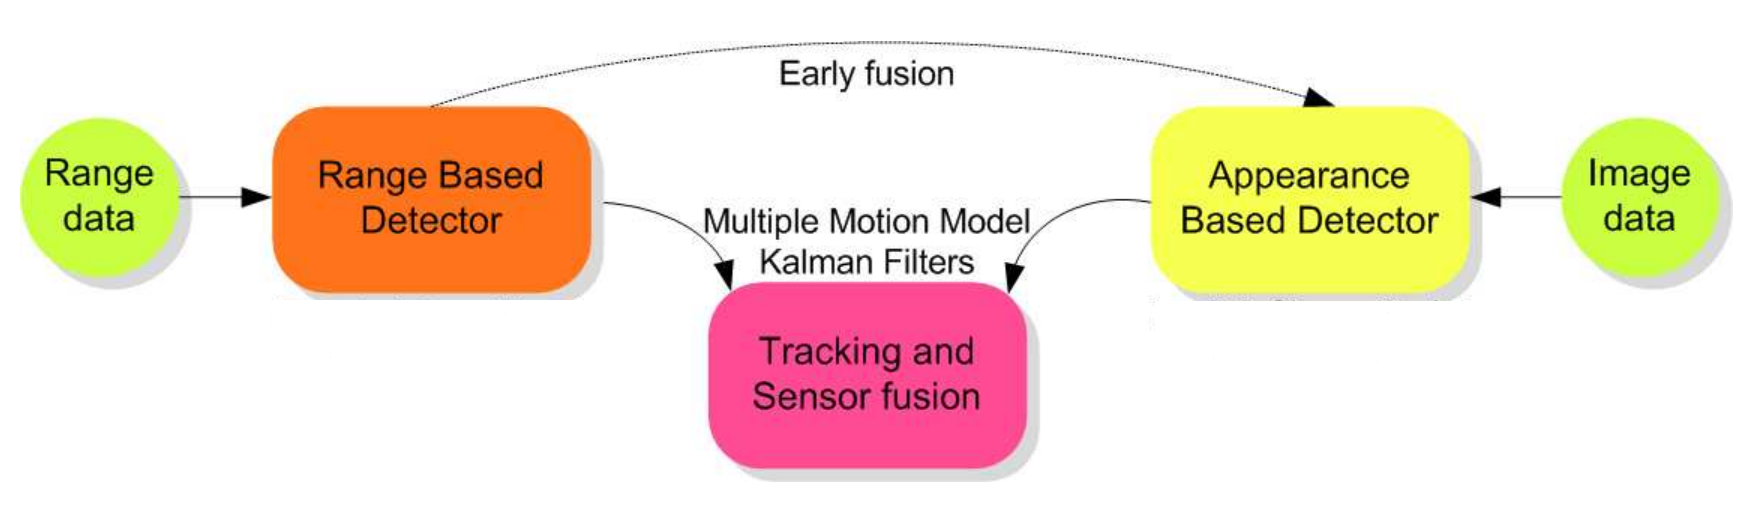
\includegraphics[width=0.99\textwidth]{capstate/imgs/multimodal.png}
	
	\caption{ Overview of the multi-modal approach. }
	\label{fig:basket}
	
\end{figure}

Utilizing a multiple motion model and Kalman filters it is possible to consolidate both range and image data. This process is called sensor fusion. By incorporating ranged based information in image data it is possible to have augmented perception of the surroundings. With the ability to have basic cognitive process of the environment, it is possible to detect and track objects in motion.

 




\chapter{Experimental Infrastructure}

In this section, the hardware and frameworks used for this thesis will be described. The hardware used was mainly the ATLASCAR 2 and its sensors: two SICK LMS151 \gls{lidar}, one SICK LD-MRS \gls{lidar} and a PointGrey Zebra 2 Camera. The central framework that receives messages from the sensors is \gls{ros}. This data will be processed using the \gls{opencv} for images, and several libraries will be used for the range-based sensors, such as the \gls{pcl} and \gls{mtt}. 

\section{ATLASCAR 2}

The ATLASCAR 2 is based in the platform of the 2015 Mitsubishi i-MiEV, a full electric vehicle. The battery that powers the engine is the same powering the camera and the sensors. The main characteristics of the car are in table \ref{tab: MiEV technical} (\cite{MITSUBISHIMOTORS}). 

\begin{figure}[htp]
	
	\centering
	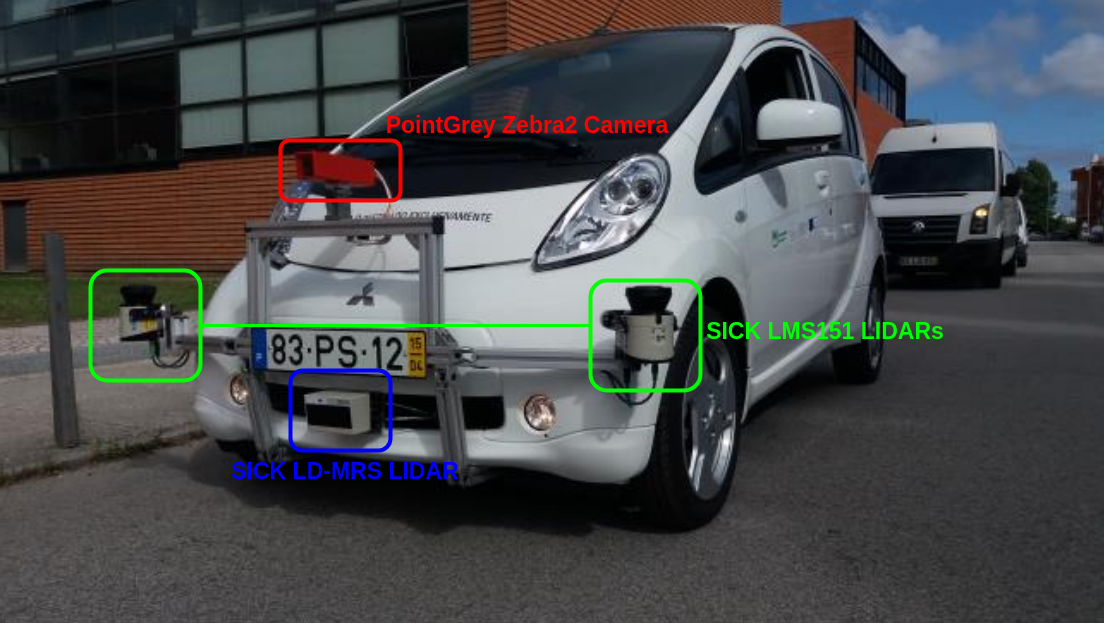
\includegraphics[width=.9\textwidth]{capexp/imgs/atlascar2.png}\hfill
	
	\caption{The ATLASCAR 2 based on the Mitsubishi i-MiEV platform equipped with a camera and several LIDAR sensors}
	\label{fig:imiev}
	
\end{figure}

\begin{table}[!h]
	\centering
	\caption{Mitsubishi i-MiEV technical specifications}
	\label{tab: MiEV technical}
	\begin{tabular}{lcc}
		Characteristic & Unit & Value\\
		Wheelbase & mm & 2550\\
		Track (Front/Rear) & mm & 1310/1270 \\
		Vehicle weight & kg  & 1450 \\
		\hline
		Engine & -- & Electric \\
		Electric energy consumption & Wh/km & 135 \\
		Electric range (NEDC)  & km & 150 \\
		Maximum speed & km/h & 130 \\
		Minimum turning radius & m & 4.5 \\
		Max. Power output & kW & 49 \\
		Max. torque & Nm & 180 \\
		\hline
		Traction battery type & -- & Lithium-ion battery \\
		Traction battery voltage & V & 330 \\
		Traction battery energy & kWh & 16 \\
		Regular charging (AC 230V 1 phase) 8A & hrs & 10 \\
	\end{tabular}
\end{table}

\section{Sensors}

The sensors equipped in the ATLASCAR 2 are two SICK LMS151 \gls{lidar}, a SICK LD-MRS \gls{lidar} and a PointGrey Zebra 2 Camera. It is of most importance for the ATLASCAR 2 to have this sensors to be capable of perception. The sensors have been mounted in the front of the car in an aluminum infrastructure designed by \cite{Correia2017}. These devices are connected to a network switch installed in the car to which a computed can be plugged to receive the data from the sensors.

\subsection{SICK LMS151 LIDAR}

The SICK LMS151 (figure \ref{fig:sicklms}) is a \gls{lidar} sensor designed to be used in outdoors. It is a planar infrared scanner with a large planar aperture angle often used in robotics and in \gls{ad} fields for its high scanning frequency and operating range. This scanner is also able to scan distances through fog, glass and dust (multi-echo technology). This scanner is provided with an Ethernet TCP/IP interface with high data transmission rate. \cite{SICK}

\begin{figure}[htp]
	
	\centering
	\hfill
	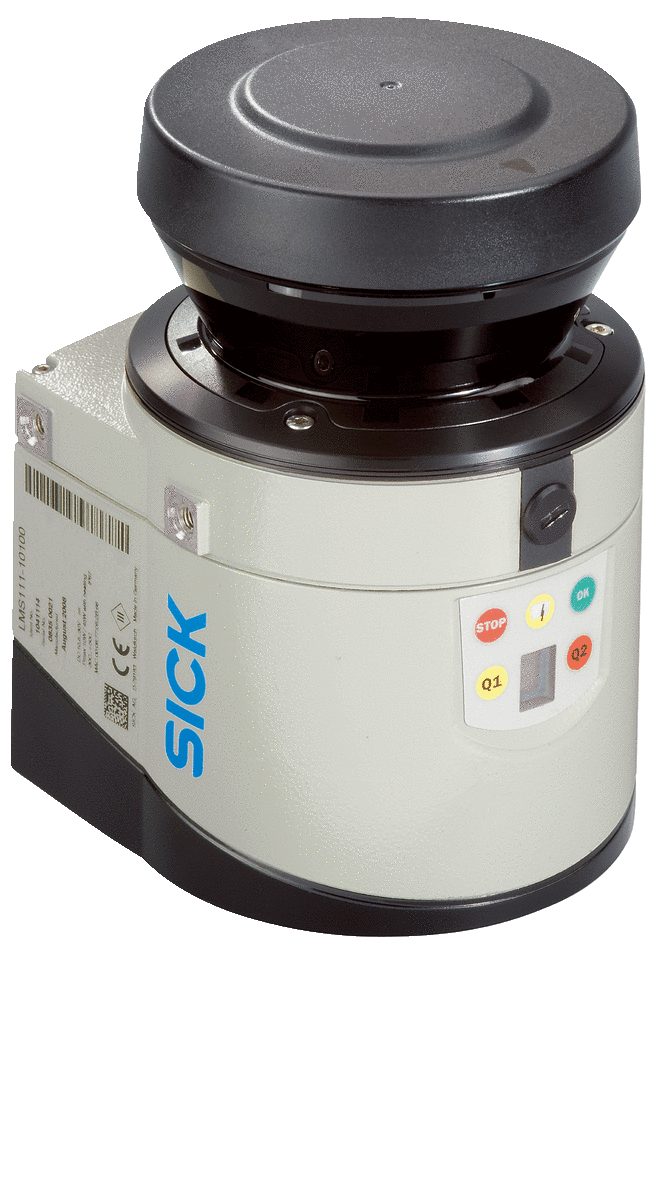
\includegraphics[width=.3\textwidth]{capexp/imgs/sicklms}\hfill
	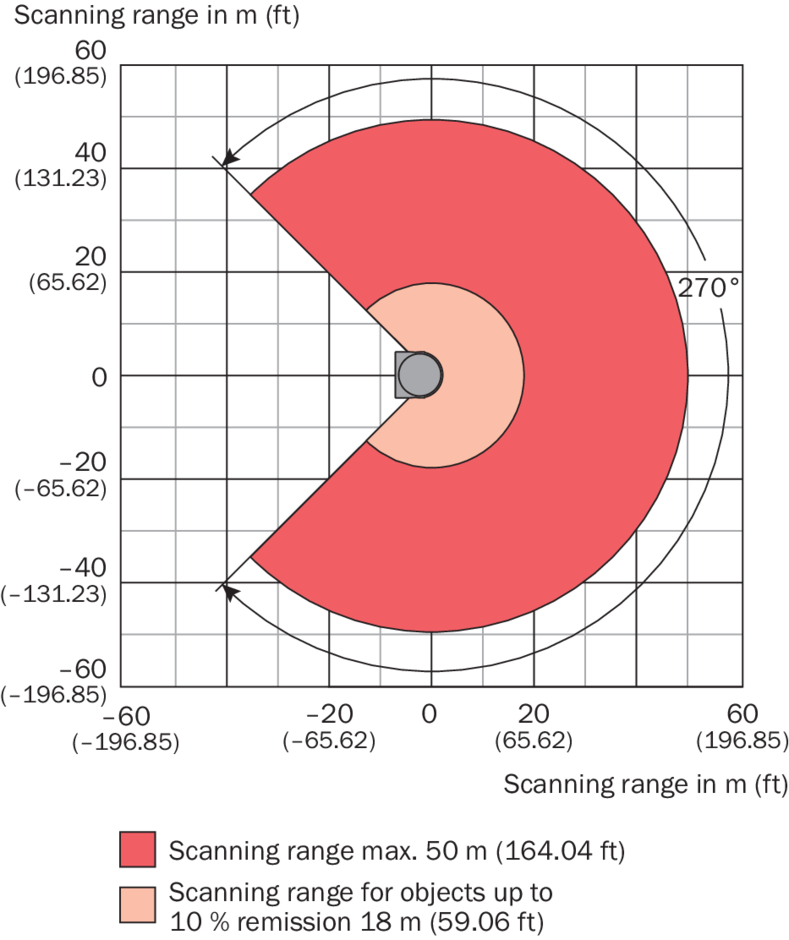
\includegraphics[width=.5\textwidth]{capexp/imgs/sicklms2}\hfill
	
	\caption{The SICK LMS151 LIDAR and its operating range}
	\label{fig:sicklms}
	
\end{figure}

\begin{table}[!h]
	\centering
	\caption{SICK LMS151 specifications}
	\label{tab: sicklmsspecs}
	\begin{tabular}{ll}
		\hline
		Field of application & Outdoors\\
		Laser Class & 	1 (IEC 60825-1:2014, EN 60825-1:2014) \\
		Aperture Angle & 270$^{\circ}$ \\
		Scanning frequency & 25 Hz / 50 Hz \\
		Angular resolution	& 0.25$^{\circ}$ / 0.5$^{\circ}$ \\
		Operating range	& 0.5 m ... 50 m \\
		Max. range with 10 \% reflectivity & 18 m \\
		Amount of evaluated echoes & 2 \\
		Data transmission rate & 10/100 MBit/s \\
		\hline
	\end{tabular}
\end{table}

For this project, the SICK LMS151 will operate at 50 Hz with an angle increment of 0.5$^{\circ}$ between readings. Each message will transmit a total of 540 points per scan in polar coordinates $(r,\theta)$. \cite{SICK}

\subsection{SICK LD-MRS LIDAR}

The SICK LD-MRS (figure \ref{fig:sickldmrs}) is a \gls{lidar} sensor also designed to be used in outdoors. It features 4 planar infrared scanners with 0.8$^{\circ}$ vertical aperture angle between each plan, offering tri-dimensional point clouds. It provides high scanning frequencies and long operating range up to 300 meters. This scanner is also provided with an Ethernet TCP/IP interface with high data transmission rate (\cite{SICKa}).

\begin{figure}[htp]
	
	\centering
	\hfill
	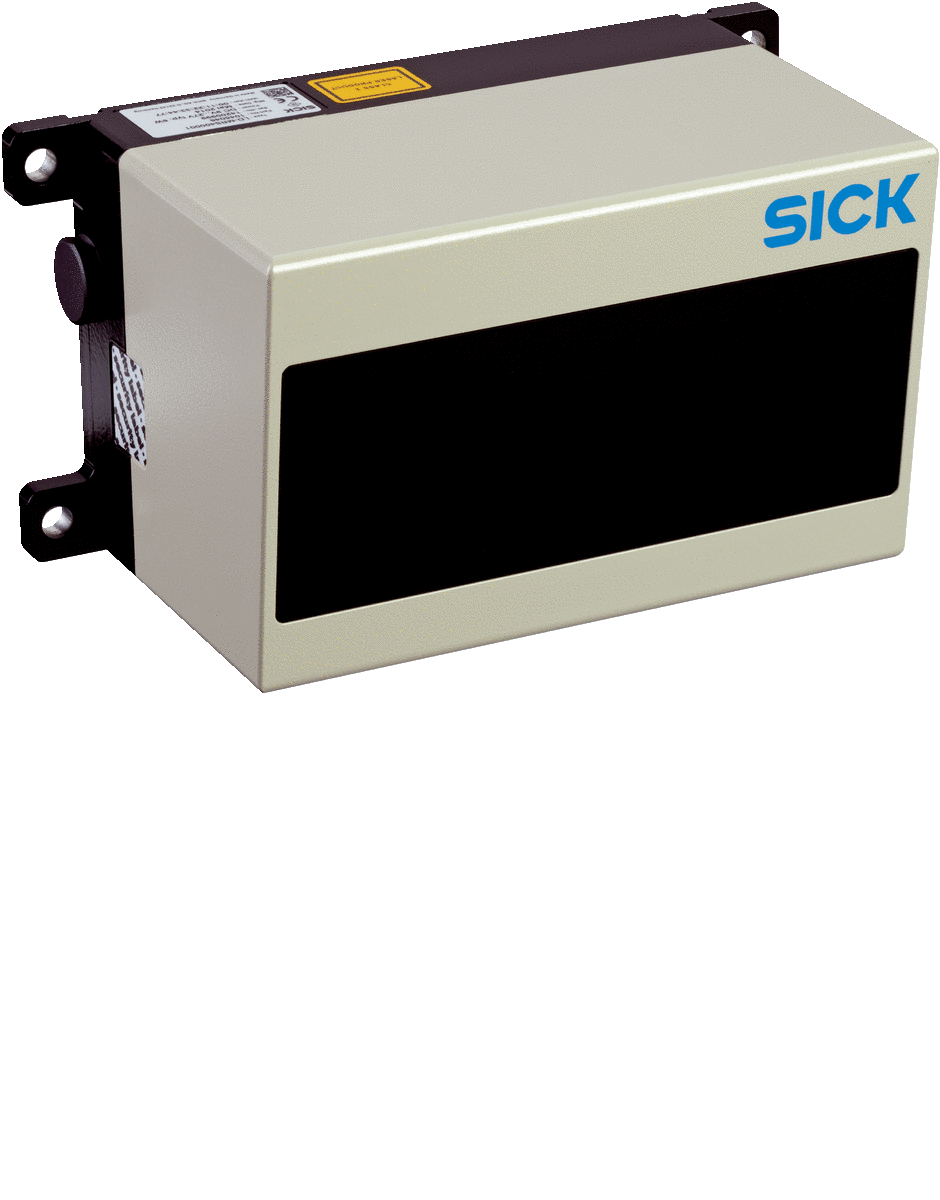
\includegraphics[width=.4\textwidth]{capexp/imgs/sickldmrs}\hfill
	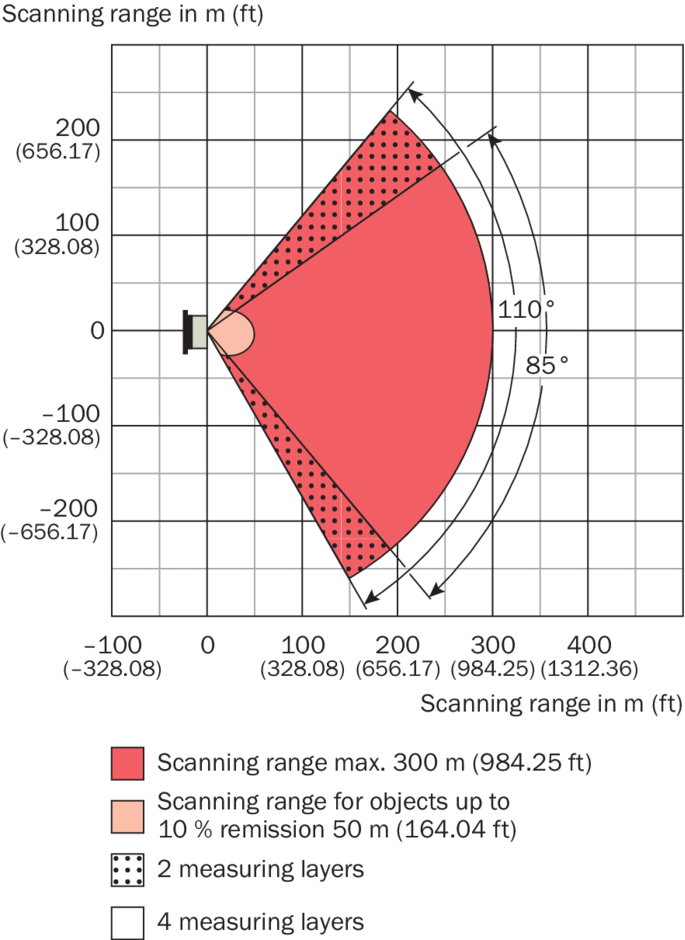
\includegraphics[width=.5\textwidth]{capexp/imgs/sickldmrs2}\hfill
	
	\caption{The SICK LD-MRS LIDAR and its operating range}
	\label{fig:sickldmrs}
	
\end{figure}

\begin{table}[!h]
	\centering
	\caption{SICK LMS151 specifications}
	\label{tab: sickldmrsspecs}
	\begin{tabular}{ll}
		\hline
		Field of application & Outdoors\\
		Laser Class & 	1 (IEC 60825-1:2014, EN 60825-1:2014) \\
		Scanner Planes & 4 measuring planes \\
		Aperture Angle & 85$^{\circ}$  \\
		Total Aperture & 110$^{\circ}$\\
		Scanning frequency & 12.5 Hz / 50 Hz \\
		Angular resolution	& 0.125$^{\circ}$ / 0.25$^{\circ}$ / 0.5$^{\circ}$ \\
		Operating range	& 0.5 m ... 300 m \\
		Max. range with 10 \% reflectivity & 50 m \\
		Amount of evaluated echoes & 3 \\
		Data transmission rate & 100 MBit/s \\
		\hline
	\end{tabular}
\end{table}

For this project, the SICK LD-MRS will operate at 50 Hz with an angle increment of 0.5$^{\circ}$ between readings. Each message will transmit a total of 200 points per scan in polar coordinates $(r,\theta)$ for each plan. Since this scanner offers four planar scans, the final point cloud will total 800 points (\cite{SICKa}).

\subsection{PointGrey Zebra 2 Camera}

The PointGrey Zebra 2 Camera (figure \ref{fig:pointgrey}) is a high resolution camera with a Sony ICX274. It also features a GigE PoE Interface and it is highly configurable to fulfill any particular utilization needs (\cite{PointGrey}). The camera is inserted in a case made with 3D printing and designed by \cite{Correia2017}.  Other relevant specifications are found in table \ref{tab: pointgreyspecs}. 

\begin{figure}[htp]
	
	\centering
	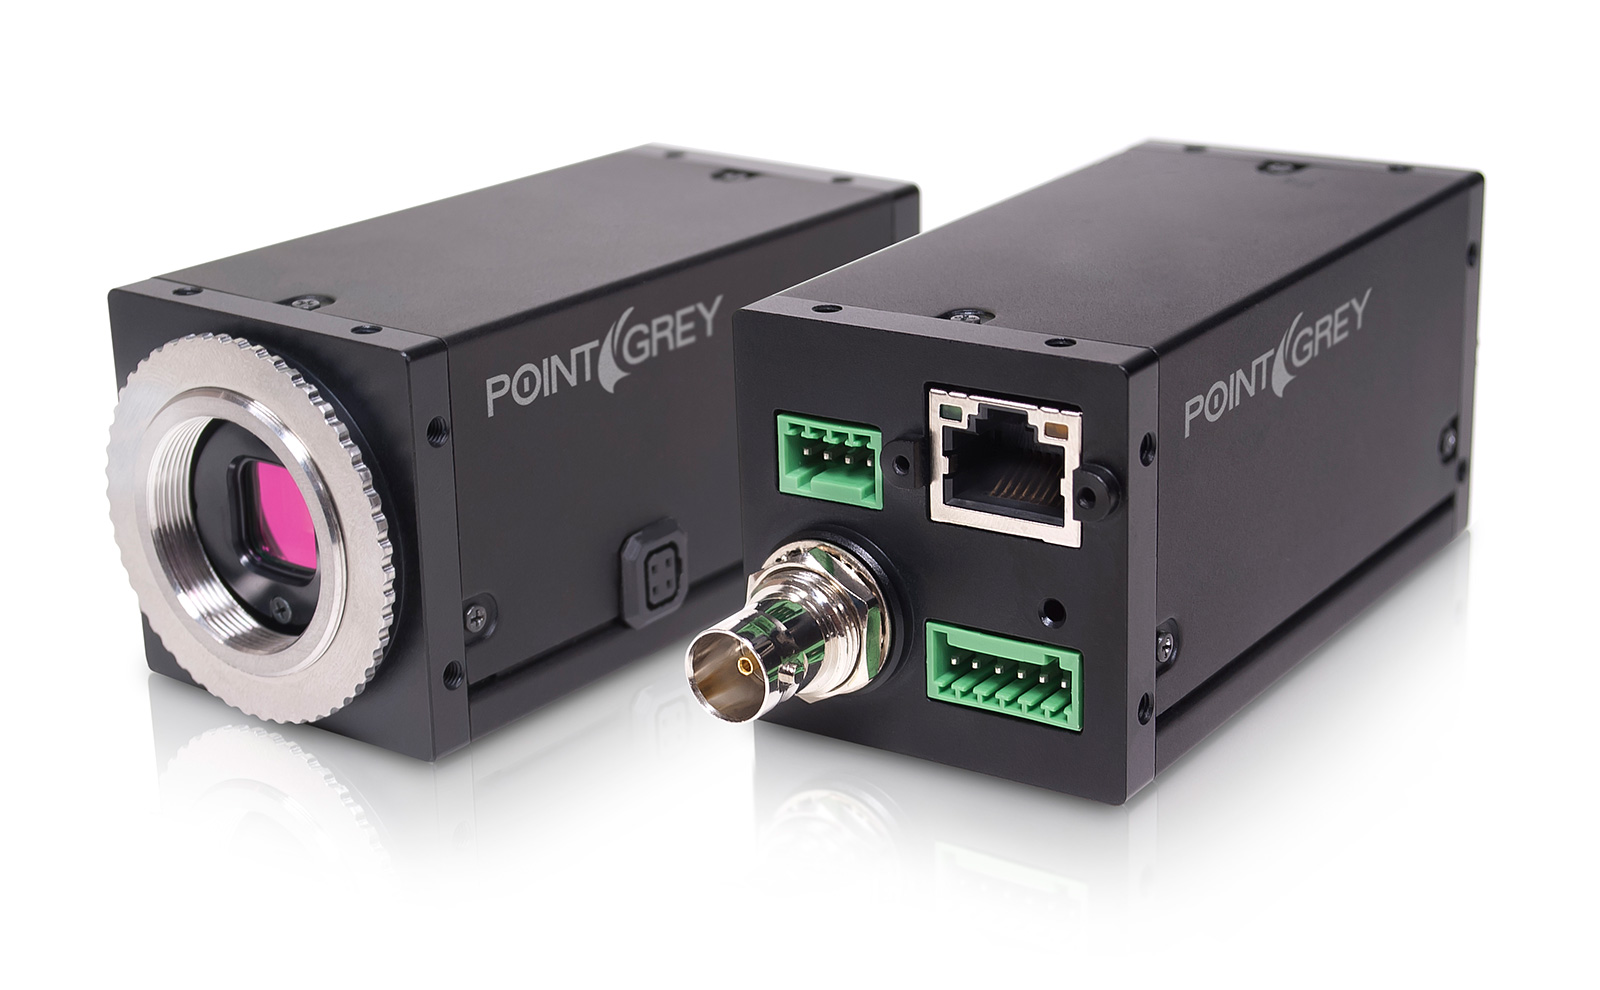
\includegraphics[width=.6\textwidth]{capexp/imgs/pointgrey}
	
	\caption{The PointGrey Zebra 2 Camera}
	\label{fig:pointgrey}
	
\end{figure}

\begin{table}[!h]
	\centering
	\caption{PointGrey Zebra 2 Camera specifications}
	\label{tab: pointgreyspecs}
	\begin{tabular}{ll}
		
		\hline
		Resolution & 1624 x 1224\\
		Max. Frame Rate & 25 FPS with HD-SDI \\
		Megapixels & 2.0 MP \\
		Chroma & Color\\
		Sensor & Sony ICX274 CCD \\
		Image Buffer &	32 MB\\
		Interface &	GigE PoE, HD-SDI\\
		
		\hline
	\end{tabular}
\end{table}

Working at maximum resolution and frame rate would saturate the network bandwidth and increase image processing times. In this project the camera's frame rate is set at 7.5 FPS so that a balance between image quality and processing optimization can be accomplished.


\section{Software}

In this section it will be discussed the software used in this dissertation. The base architecture of this dissertation is centered in the \gls{ros} framework. Many \gls{ros} tools and features are used such as Rviz, rosbags, roslaunch and rosrun. Two main nodes are to be developed in this work: the camera calibration package node (previously developed by \cite{VieiradaSilva2016}) and the labelling node. The handling of data from the sensors was done using \gls{pcl}, \gls{mtt}, 
and the image processing was performed with \gls{opencv} libs. All software was programmed with C++.

\section{ROS}
The central framework in the ATLASCAR 2 is based on \gls{ros} Kinect on Ubuntu 16.04.

The Robot Operative System, although not an operating system, operates as a robotics middleware. \gls{ros} offers open-source services designed for developers that need hardware abstraction and low-level device control. Architectures in \gls{ros} are centered in applications called rosnodes which communicate with each other creating a graph of  message-passing processes. 

With \gls{ros} it is possible to receive data packets and transform them in messages that contain data from the sensors. It is possible to manipulate this data using \gls{ros} nodes and other tools. 

\subsection{Rviz}
Rviz is the standard \gls{ros} tool for 3D visualization. %falar mais um pouco sobre o rviz%

The Rviz is one of the most important tools as it will be used to visualize data from the ATLASCAR 2 either directly in real-time by connecting a computer to the car or in rosbags. It will also serve as a debugging tool in which pointcloud values can be analyzed (\cite{ROSWiki}).

\subsection{Rosbag}

A rosbag is a file in \gls{ros} which contains messages saved from past events. While connected directly to a device, or several devices, multiple topics can be subscribed at once to be recorded into a rosbag. 

The advantage of rosbags in this dissertation is to simulate the working environment of the ATLASCAR 2 without actually being in it. Several rosbags were recorded throughout the process of development in this project, either of calibration or for detection, tracking and labeling purposes. 

In \gls{ros}, the rosbag package contains a set of tools for recording from and playing back to \gls{ros} topics. It is intended to be high performance and avoid deserialization and reserialization of the messages. It also features command line tools for working with bags as well as code APIs to read/write and manipulate bags (\cite{ROSWikia}).

\subsection{Roslaunch}
The roslaunch files are used as a tool for easily launching multiple \gls{ros} nodes. A roslaunch file sets up a roscore (os \gls{ros} master), sets parameters on the Parameter Server, and can also execute other roslaunch files. 

It includes options to automatically re-spawn processes that have already died. The roslaunch takes in one or more XML configuration files (with the .launch extension) that specify the parameters to set and nodes to launch.

For example, a rosbag can be given as parameter to the roslaunch which opens the Rviz with a previous defined configuration to visualize the data from that rosbag.

In this project, roslaunch files are optimal to set up calibration values before launching the Rviz and the nodes that process the data from the \gls{lidar}s and the camera. The transformations between device frames are set up using roslaunch files and static transform publishers implemented by \gls{ros}. 

The roslaunch files are also advantageous to set up the multiple drivers needed to bring up the several devices equipped in the ATLASCAR 2. Since the sensors are connected to a network switch, the parameters given in the driver's roslaunch file are the IP addresses of each of the devices. The drivers will then receive packets from the sensors and remap them into the \gls{ros} format.

\section{LAR Toolkit}

The \gls{lartk} is a software suite developed by members of the \gls{lar}. The projects involved in the \gls{lartk} are based in the development of robotic solutions namely for the ATLAS project. The toolkit is constituted by a set of packages, in which 2 main packages will be used for this disseration: the multi-sensor calibration package and the \gls{mtt} package.

\subsection{Multi-sensor calibration package}

The multi-sensor calibration package is a package developed by \cite{VieiradaSilva2016}. The package contains a \gls{gui} used to calibrate the several sensors in the ATLASCAR 2. The package was initially developed for the ATLASCAR 1, and it was further used into the ATLASCAR 2 since the sensors were almost the same.

The calibration package features a graphical user interface in which several sensors can be selected to be calibrated. The available devices are the SICK LMS151 and SICK LD-MRS mounted in the ATLASCAR 2, PointGrey cameras, Microsoft Kinects, the SwissRanger SR4000 and the Velodyne VLP16 used in the ATLASCAR 1.


\subsection{Multi Target Tracking (MTT)}

The \gls{mtt} library is a set of methods and strategies developed by \cite{SoaresDeAlmeida2016a} specially designed for the ATLASCAR project with the goals to use the planar scanners to obtain perception about objects captured in the \gls{lidar}s. The ATLASCAR2 is equipped with scanners that send data in a message format. 

The \gls{mtt} is capable of receiving these messages and break them in smaller groups. This process is called clustering. Clustering separates all objects found in a scan and returns their position. The clustering of data is an important step in the development of this dissertation as it facilitates the detection and tracking of objects in space. 

The clustering algorithm of the \gls{mtt} library segments the received pointclouds using a predefined distance as threshold. Each set of points in the clusters are assumed as possible targets of interest.

The \gls{mtt} then associates the targets found to a linked list of objects where the full description of the objects are stored. This list is later used to create a motion model where the estimated position of the objects and its velocity is calculated. 

Some objects may become occluded, for example when a car passes in front of another. The \gls{mtt} estimates the position of the occluded objects by creating a motion model using their velocity and so it is possible to track objects while they are out of the field of view but still in the surroundings.

The \gls{mtt} operates around targets. Targets keep information about the object and its velocity plus their position and obstacle lines.

\section{\gls{pcl}}

The \gls{pcl} is a library that implements methods to process pointcloud data. The \gls{pcl} framework contains numerous state of the art algorithms including filtering, feature estimation, surface reconstruction, registration, model fitting and segmentation (\cite{PointCloudLibrary2018}). Some of these algorithms are used throughout this thesis an were also used by the \gls{mtt} library.
It is important to use the \gls{pcl} in this project as it works with a lot of data from \gls{lidar} sensors at the same time. 



 









\chapter{Improvement of the Calibration Process in ATLASCAR2}

Using sensors to recognize the environment is of most importance for vehicles to become fully autonomous. A car equipped with several sensors needs to know the position of each sensor so that the readings can be aligned and exact perception can be obtained. 

One of the main tasks for this dissertation is to be improve the extrinsic camera calibration process. Multi sensor calibration in ATLASCAR 2 is done using a ball as a target. One of the limitations of the approach in \cite{VieiradaSilva2016} is the use of filtering the image using HSV values to detect the ball.

While moving the ball around the sensors, a point cloud of ball centers is created for each sensor. These point clouds are aligned so that the estimate pose of each sensor can be obtained using an arbitrary sensor as reference.

\section{New Ball Detector Algorithm}

This section describes the progress introduced in the development of the ball detector.

\begin{figure}[htp]
	
	\centering
	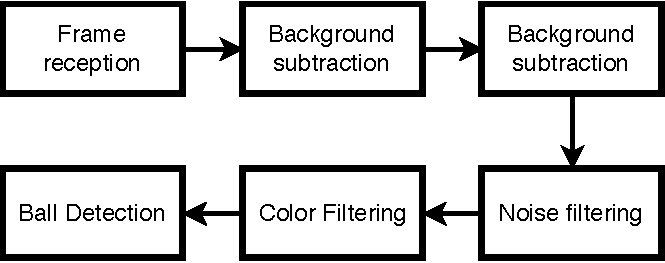
\includegraphics[width=0.8\textwidth]{capcalib/imgs/calib_implementation.pdf}
	
	\caption{New ball detection algorithm simplified diagram}
	\label{fig:ball_diagram}
	
\end{figure}

The ball detection upgrade begins by retrieving the video stream frames from the PointGrey camera. The image obtained was worked in a rosbag used for testing in order for the development to be made outside the ATLASCAR 2. The ball used in the tests is shown in figure \ref{fig:ball}. 

\begin{figure}[htp]
	
	\centering
	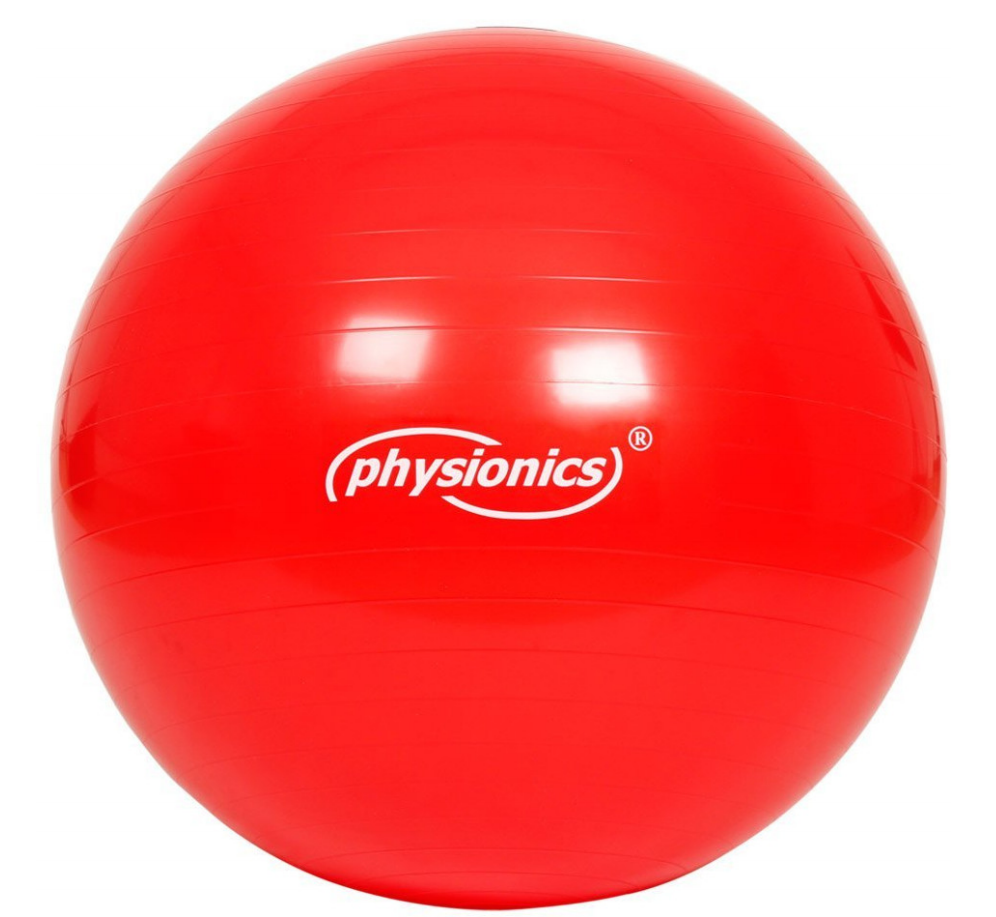
\includegraphics[width=0.4\textwidth]{capcalib/imgs/ball.png}
	
	\caption{Ball used for calibration testing}
	\label{fig:ball}
	
\end{figure}

To acquire the images, the ball detector node creates a subscriber to get messages from the camera topic. \gls{ros} subscribers take the message in the topic and send it to a callback function in order to it to be processed. After obtaining information from the camera's message, it is needed to convert the RGB values into the \gls{hsv} color space so that the image can be easily manipulated.

\subsection{Background Subtraction}

The first thing to do with the frames is to apply background subtraction. The vehicle is supposed to be still when the calibration process is being done, so the background subtraction is a good method to apply.

\begin{figure}[h!]
	
	\centering
	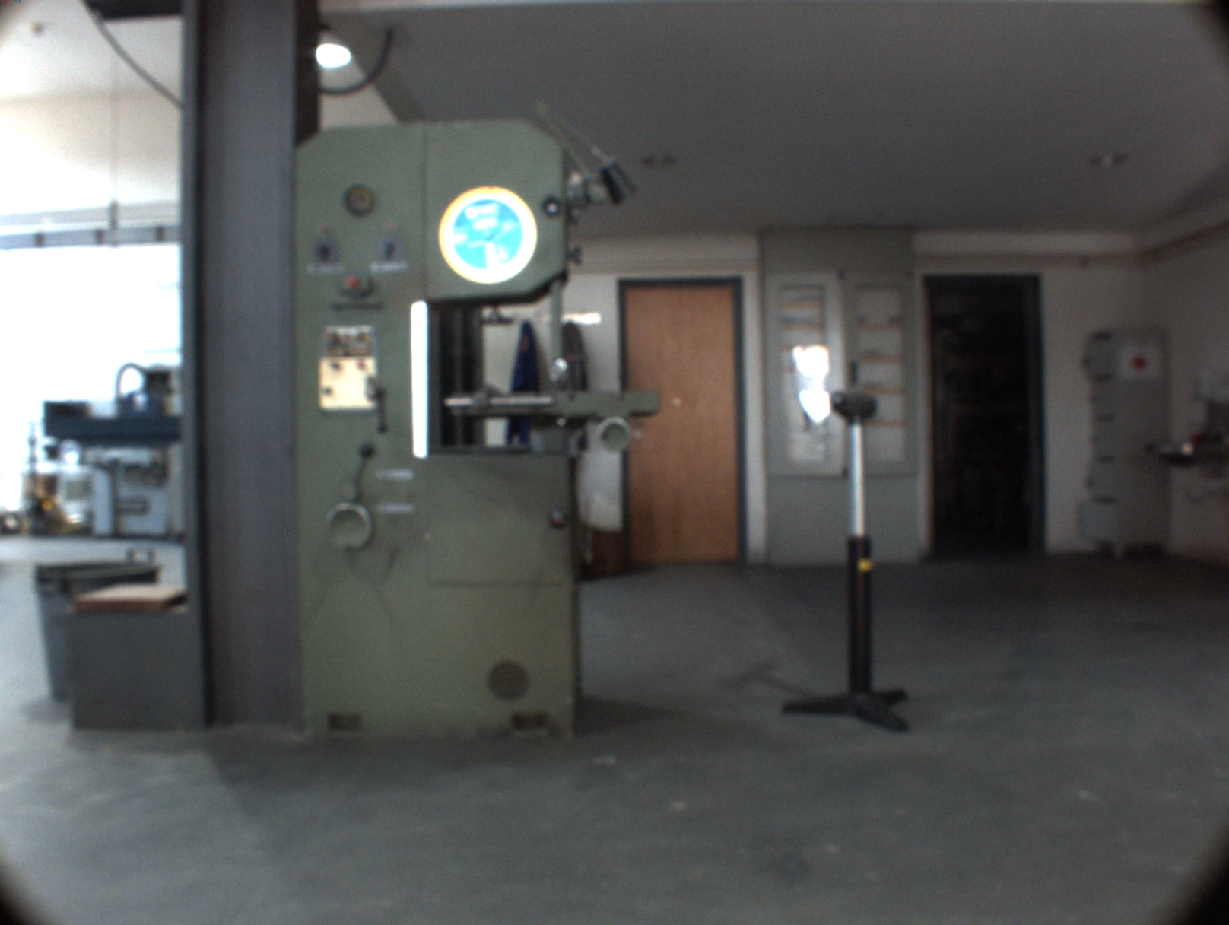
\includegraphics[width=0.65\textwidth]{capcalib/imgs/background.png}
	
	\caption{Background in test rosbag used for testing}
	\label{fig:background}
	
\end{figure}

When the capture starts, the first received frame will be the default background (see figure \ref{fig:background}). The background removal is a process used in many vision based applications with static cameras, in which a frame is captured and defined as the background of a sequence of images. Therefore, when an objects enters the scene (figure \ref{fig:balltest}), by subtracting the background with the actual frame it is possible to detect easily where the object is (\cite{OpenCV}).

\begin{figure}[htp]
	
	\centering
	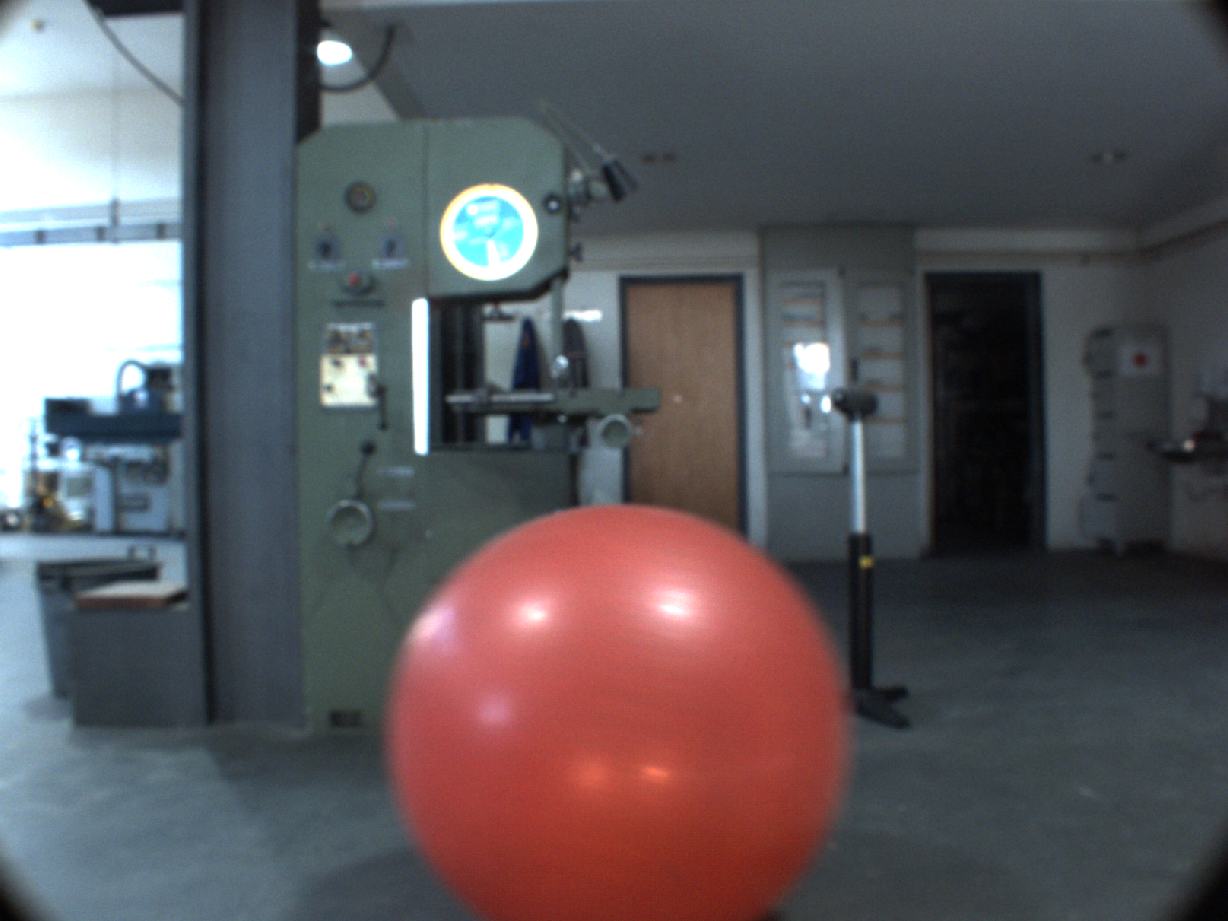
\includegraphics[width=0.5\textwidth]{capcalib/imgs/ball_test.png}
	
	\caption{Frame with ball rolling in front of the camera}
	\label{fig:balltest}
	
\end{figure}

In simple words, background subtraction extracts the foreground from the static background. Most times, the background is modified by applying Gaussian blur to it. When subtracting the foreground with the background, a value is obtained for each pixel.

In most cases the pixel values will not get to zero because of minor changes to the background (caused by shadows) which need to be ignored. In the resulting image a threshold is applied. If a pixel presents a value under the threshold, then it is set to zero (black), otherwise it is set to one (white). In the end, it is obtained a binary image containing some noise due to shadows or other lightning changes, and potentially an area with more concentrated white values where new objects appear. The result is a binary image as seen in figure \ref{fig:ballnoise}.


\begin{figure}[htp]
	
	\centering
	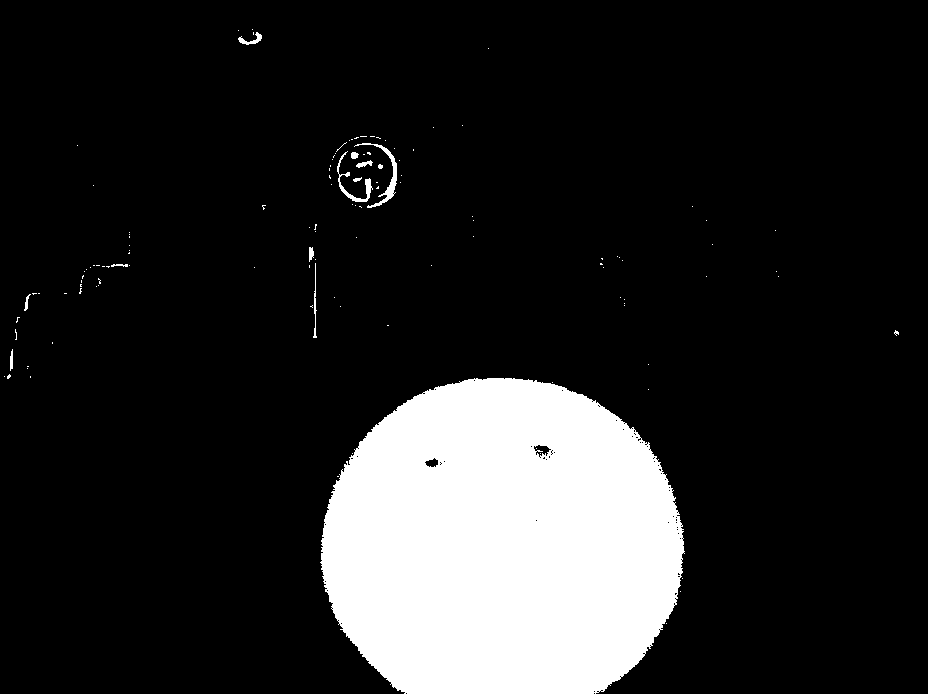
\includegraphics[width=0.5\textwidth]{capcalib/imgs/noise.png}
	
	\caption{Background subtraction result with noise}
	\label{fig:ballnoise}
	
\end{figure}

\subsection{Noise Filtering}

After the background removal technique is applied, the resulting image may possibly contain some noise. Some pixels may be left white in the background due to lightning changes when the ball passes in front of the camera. These white pixels are noise and must be removed.

An erosion algorithm is implemented where for each pixel the neighbor pixels are counted. The image is processed left-to-right, top-to-bottom, so the matrix corresponding to the frame is iterated throughout its lines. A counter is added to check if the previous pixels contained white pixels (with value of 1). 

\begin{figure}[htp]
	
	\centering
	\includegraphics[width=0.5\textwidth]{capcalib/imgs/neighpixel.pdf}
	
	\caption{Neighbor pixels used in the algorithm where grey pixels represent the kernel and the pixel P represents the pixel being processed}
	\label{fig:neigh_cnt}
	
\end{figure}

As the kernel is scanned over the image, the algorithm computes the minimal pixel value overlapped by the kernel and replaces the image pixel under the anchor point with that minimal value (\cite{OpenCV2.4.13.6documentation}). The result is the image in figure \ref{fig:balldetect}.

\subsection{Color Filtering}

After the noise filtering, the ball stands out in the image. The next step is to separate the ball using color filtering. This step is necessary to make the detection usable when a person appears in the image to displace the ball. This way, the person will not appear in the resulting image.

The selected color by default is red. To set the ball color, the user needs to click in the ball to capture its hue. A mouse event is triggered and an handler function is called. The handler localizes the mouse click and retrieves the RGB values of the pixel in those coordinates. These values are converted to a hue value of the \gls{hsv} color space. The selected hue is the color used to filter the ball from the rest of the image. By applying certain thresholds it is possible to define an interval of color. The image will then be filtered by an interval centered in that hue value and the ball is now filtered from the rest of the image. 


\subsection{Bounding Box}

A bounding box is drawn around the ball if there is a number of white pixels bigger than a predefined threshold. To do this, the image is iterated like in this erosion phase, left-to-right and top-to-bottom. The algorithm saves the coordinates of all white pixels. An average $x$ and $y$ are calculated, finding the ball center in the image. The size of the bounding box is given by how much white is in an specific area. Supposing there is a possibility of a white pixel to appear as noise, that pixel will have low weight in the algorithm considering that the pixels around it are black. Therefore, white pixels gathered in a larger area have greater weight. Hence, the width and height of the bounding box are given by the maximum distance between the pixels with higher weight.


\begin{figure}[htp]
	
	\centering
	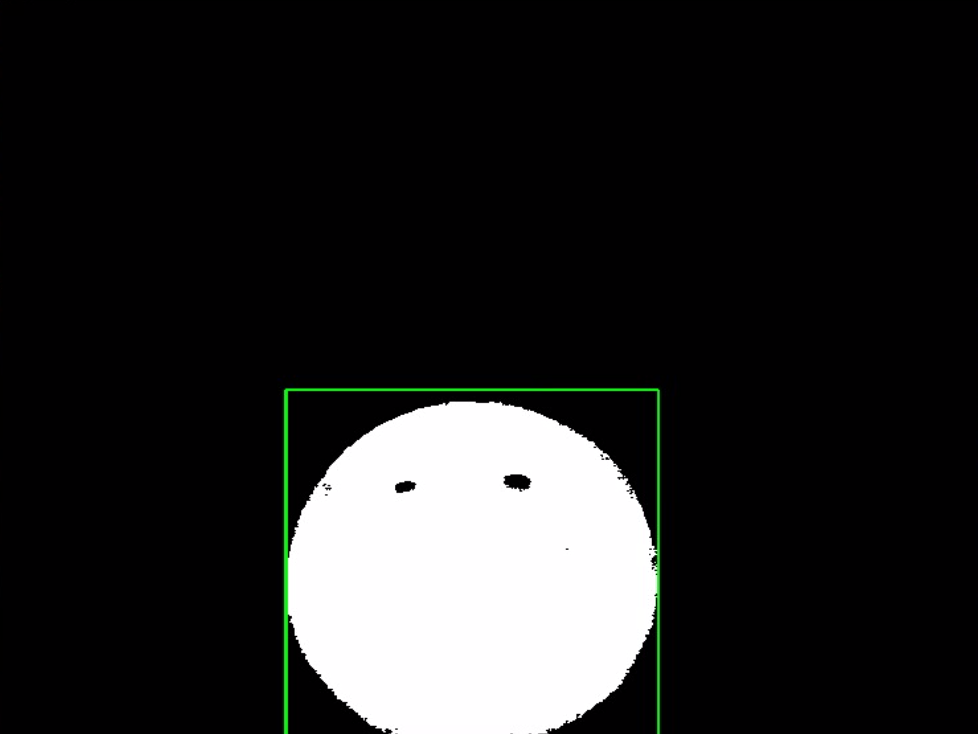
\includegraphics[width=0.7\textwidth]{capcalib/imgs/ball_detect.png}
	
	\caption{Ball detected with bounding box}
	\label{fig:balldetect}
	
\end{figure}

\section{Modifying the calibration package}

The calibration package used to calibrate the several sensors in ALTASCAR 2 uses multiple nodes, one for each kind of sensor. The camera node in the package is called \texttt{point\_grey\_camera} and it uses the source file \texttt{point\_grey\_camera.cpp}. This file was modified in order to add the implemented features into the calibration package. 

The \texttt{point\_grey\_camera} node receives the camera image by subscribing to the camera topic with \gls{ros}. The camera sends images in a \gls{ros} message format to be interpreted and processed by a callback function. The image processing algorithm follows the steps explained in the previous section. After performing the ball detection, the center of the bounding box matching the center of the ball is retrieved. The ball center is published into the calibration package main node \texttt{calibration\_gui}.

The radius of the ball is passed as an argument so it is possible to calculate the distance from the camera to it. The centroids are obtained with a method based on the circle radius and they are published as \texttt{PointStamped} \gls{ros} points to be presented in the calibration \gls{gui}. 















 


\chapter{Object Detection, Tracking and Labelling}

The main task of this dissertation is focused on the detection, tracking and labeling of objects in motion found in the field of view of the several sensors equipped in ATLASCAR 2. In this chapter it will be succinctly explained how these features were implemented. 

Firstly, it will be described how the detection and tracking in the image is performed. In the image tracking phase happens also the labelling phase and the creation of dataset files and image templates. 

Secondly, the implementation of the tracking of multiple targets with ranged based sensors will be explained. To make this step possible, the MTT library designed by Almeida \cite{SoaresDeAlmeida2016a} was used. The MTT library contains methods of perception and planar object detection. 

Lastly, the multi-modal approach will be used where both data from the images and the LIDARs will be assembled and a single perception unit will be created. With this conceptualization, it is possible to detect, track and label objects easily in the ATLASCAR 2.

The image sequences and laser scan data obtained for the development of this stage of the dissertation were recorded into rosbags using the ATLASCAR 2 using the sensors it has. The rosbags were recorded in October 17, 2017, in the afternoon. Two rosbags were recorded:

\begin{itemize}
	\item The first rosbag was recorded while leaving Departamento de Engenharia Mec\^anica at Universidade de Aveiro. The car travelled around the campus and visited the Alboi neighbourhood.
	\subitem In this bag there are cars, vans, cyclist and pedestrians. It is a bag where the car also runs into slopes. It is a rosbag with more detail which was used later in the project.
	\item The second rosbag starts at Alboi where the last rosbag stopped. The car follows a path into the A25 highway until the first exit.
	\subitem There are mostly cars in this one and it was a good rosbag to start with some tests in tracking objects.
\end{itemize} 

\section{Image Tracking}

The development of object detection, tracking and labelling starts by processing and analyzing the image sequences. A labelling node was created in ROS where the features in this chapter were implemented. This node subscribes to the camera images through its rostopic. In resemblance to the calibration, the image comes encapsulated in a ROS message to be processed in a callback function. In this function the image is analyzed.

The image is converted from the ROS message format into an OpenCV format so it can be easily manipulated. As the image sequences arrive, they are stored into a queue. This queue will be used later to look back to the previous frames and back-track the object. 

\subsection{Image Labelling}

\section{Multi Target Tracking}
\chapter{Results}

This chapter presents the results of the improvement of the calibration process and object detection, tracking and labelling system.

\section{Camera Calibration}

Figure \ref{fig:gui} presents the multisensor calibration \gls{gui}. One of the SICK LMS151 \gls{lidar}s was used as point of reference for the purpose of demonstration and to have a comparator point to the camera.

\begin{figure}[htp]
	
	\centering
	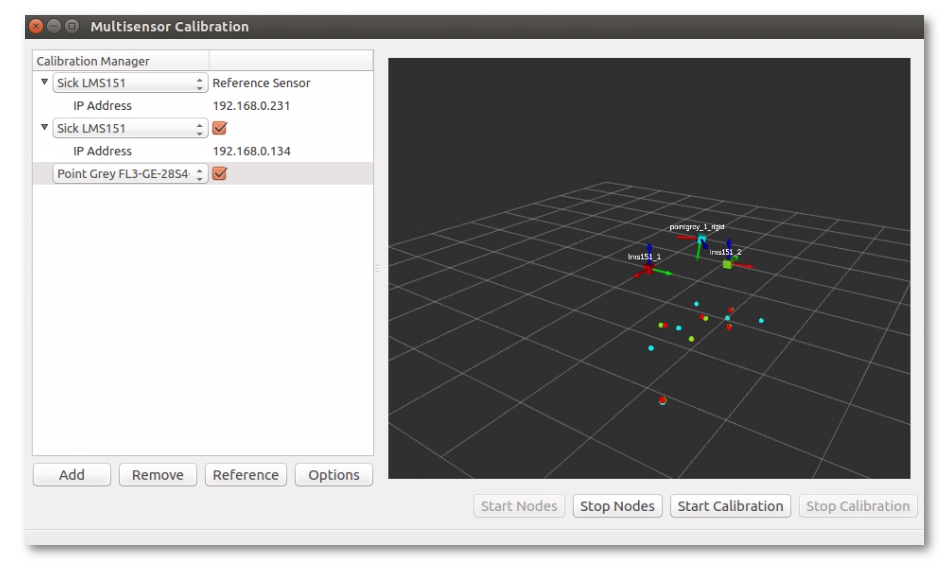
\includegraphics[width=0.9\textwidth]{capresults/imgs/gui.png}
	
	\caption{Calibration GUI with calibration result}
	\label{fig:gui}
	
\end{figure}

During the calibration procedure, the ball rolls in front of the camera and sensors. The range based sensors and the camera obtain a pointcloud of centroids of the ball during this activity. In the end, the transforms for each sensor are calculated, aligning the pointclouds of the several devices with each other. 

\begin{figure}
	\begin{center}
		\begin{lstlisting}[label={lst:calib_result}, caption={Calibration output file.},language=c++]
		-0.0563334  -0.998402 0.00440481   -1.07636
		0.997797 -0.0561436  0.0353294    1.08224
		-0.0350256 0.00638533   0.999366  0.0617893
		0          0          0          1	\end{lstlisting}
	\end{center}
\end{figure}

In listing \ref{lst:calib_result} an example output file of the calibration can be observed. The file contains a 4x4 matrix that indicates the transforms for the given sensor. Each sensor in the calibration will output its own file containing its transformation matrix relatively to the reference sensor. The reference sensor does not create a transform because it is assumed that this sensor is in the origin, unrotated. 

\section{Detection, Tracking and Labelling}

This section will present the detection, tracking and labelling results with two rosbags recorded and used for the testing of the detection, tracking and labelling algorithms. Two rosbags were recorded:

\begin{itemize}
	\item The first rosbag was recorded while leaving Departamento de Engenharia Mec\^anica at Universidade de Aveiro. The car travelled around the campus and visited the Alboi neighbourhood.
	\begin{itemize}
	\item In this bag there are cars, vans, cyclists and pedestrians. It is a bag where the car also runs into slopes. It is a rosbag with more detail which was used later in the project.
	\end{itemize} 
	\item The second rosbag starts at Alboi where the first rosbag stopped. The car follows a path into the A25 highway until the first exit.
	\begin{itemize}
	\item There are mostly cars in this one and it was a good rosbag to start with some tests in tracking objects.
	\end{itemize} 
\end{itemize} 


Each rosbag produced a dataset where the objects found were registered. Looking into the datasets can show how the algorithm behaves.

\subsection{Dataset 1 - Highway / A25}

The first dataset was produced from the highway rosbag. The rosbag duration is 3:37s (217s), has a size of 8.6 GB and includes 62352 messages.

The labelling was done using semi-automatic methods using sensor fusion and also manually by pointing and clicking on an object when the sensors don't find it. The semi-automatic methods suggest the user an object of interest and asks for a label from the user.

\begin{table}[]
	\centering
	\caption{Highway dataset annotation metrics}
	\label{tab: highwaymetrics}
	\begin{tabular}{c|c}
		\textbf{Metric}      & \textbf{Count} \\ \hline
		\textbf{\begin{tabular}[c]{@{}c@{}}Right\\ Suggestions\end{tabular}}            & 12             \\ \hline
		\textbf{\begin{tabular}[c]{@{}c@{}}Wrong\\ Suggestions\end{tabular}}            & 6              \\ \hline
		\textbf{\begin{tabular}[c]{@{}c@{}}Manual\\ Entries Saved\end{tabular}}         & 1              \\ \hline
		\textbf{\begin{tabular}[c]{@{}c@{}}Manual Entries\\ Discarded\end{tabular}}     & 0              \\ \hline
		\textbf{\begin{tabular}[c]{@{}c@{}}Maximum Objects\\ in One Frame\end{tabular}} & 1             
	\end{tabular}
\end{table}

Several objects were found in this sequence. The discarded objects or the objects wrongly suggested by the semi-automatic system are still saved but labelled as \texttt{DontCare}. Other labels used are \texttt{car}, \texttt{van}, \texttt{people}, \texttt{bicycle}, \texttt{sign} (street signs) and \texttt{misc} (miscellaneous objects in the streets like dumpsters, bushes and trees). The amount of objects found in this rosbag is listed in table \ref{tab: highwaystats}.

\begin{table}[]
	\centering
	\caption{Highway dataset object amounts}
	\label{tab: highwaystats}
	\begin{tabular}{c|c|c|c|c|c|c|c|c}
		\textbf{Label} & \texttt{car} & \texttt{van} & \texttt{people} & \texttt{bicycle} & \texttt{sign} & \texttt{misc} & \texttt{DontCare} & \textbf{total} \\ \hline
		\textbf{Count} & 7            & 1            & 0               & 0                & 4             & 1             & 6                 & 19            
		 
	\end{tabular}
\end{table}

As this sequence presents few objects at a time, most semi-automatic suggestions were accepted. The semi-automatic system works better in areas with reduced movement so the readings of the sensors are more accurate.

\subsection{Dataset 2 - Aveiro City Urban Area}

The second dataset was generated from the rosbag at an urban area in Aveiro city. The rosbag duration is 7:06s (456s), has a size of 18.0 GB and includes 135379 messages. 

The labelling in this rosbag was done using the semi-automatic methods and the manual methods separately. The reason for this is to compare the behavior of the semi-automatic suggestions and the manual method in a different environment.

\subsubsection{Dataset 2.1 - Semi-Automatic Method}

The dataset produced with the semi-automatic method the labelling metric listed in table \ref{tab: urban1metrics}.

\begin{table}[]
	\centering
	\caption{Urban area dataset with semi-automatic methods annotation metrics}
	\label{tab: urban1metrics}
	\begin{tabular}{c|c}
		\textbf{Metric}              & \textbf{Count} \\ \hline
		Right Suggestions            & 36                      \\ \hline
		Wrong Suggestions            & 74                      \\ \hline
		Maximum Objects In One Frame & 1                      
	\end{tabular}
\end{table}

The Urban area is a zone with high-traffic and because there are more objects (sidewalks, road boundaries, walls, etc...), the semi-automatic method is more likely to mistake an object of interest with something with no significance in the dataset scope. 

The metrics show that nearly 2 out of 3 suggestions are something that has no interest for the dataset. In table \ref{tab: urban1stats} the amount of objects found is presented.

\begin{table}[]
	\centering
	\caption{Urban area dataset  with semi-automatic methods object amounts}
	\label{tab: urban1stats}
	\begin{tabular}{c|c|c|c|c|c|c|c|c}
		\textbf{Label} & \texttt{car} & \texttt{van} & \texttt{people} & \texttt{bicycle} & \texttt{sign} & \texttt{misc} & \texttt{DontCare} & \textbf{total} \\ \hline
		Count          & 29           & 2            & 4               & 0                & 1             & 0             & 74                & 110           
	\end{tabular}
\end{table}


\subsubsection{Dataset 2.2 - Manual Method}

To test the manual method, one must click on the object and control the rosbag (pause it, go back and forward, etc...) to obtain maximum precision on the detection and tracking. 

\begin{table}[]
	\centering
	\caption{Urban area dataset with manual methods annotation metrics}
	\label{tab: urban2metrics}
	\begin{tabular}{c|c}
		\textbf{Metric}              & \textbf{Count} \\ \hline
		Entries Saved           & 89                      \\ \hline
		Entries Discarded            & 31                      \\ \hline
		Maximum Objects In One Frame & 4                 
	\end{tabular}
\end{table}

In table \ref{tab: urban2metrics} some annotation metrics are shown. Despite the high traffic zone, the metrics in the manual methods show that nearly 3 out of 4 clicks result in a good detection and tracking of the object. 

Because the annotation was done manually, it is possible to enter more than one object at the same time whereas in the semi-automatic that is not possible because when the sensors suggest an object in sight, the algorithm always outputs the object that is closer to the vehicle. In table \ref{tab: urban2stats} it is possible to see the amount of each object in this dataset.

\begin{table}[]
	\centering
	\caption{Urban area dataset with manual methods object amounts}
	\label{tab: urban2stats}
	\begin{tabular}{c|c|c|c|c|c|c|c|c}
		\textbf{Label} & \texttt{car} & \texttt{van} & \texttt{people} & \texttt{bicycle} & \texttt{sign} & \texttt{misc} & \texttt{DontCare} & \textbf{total} \\ \hline
		Count          & 63           & 10            & 10               & 2                & 1             & 3             & 31                & 120           
	\end{tabular}
\end{table}

Analyzing table \ref{tab: urban2stats} it is possible to conclude that with manual methods one can freely enter with more detail the detected objects. In comparison to the semi-automatic methods, with the manual strategy it is easier to enter objects like people and bicycles as it seems to be difficult to cluster such small objects in the given sensor data.














\cleardoublepage

\chapter{Conclusions and Future Work}

In this chapter it will be wrapped up the work done during this dissertation regarding the creating of a \gls{ros} package, implementation of the ball detection node and the labelling node. Having this conclusions as a foundation, a few related future works will be proposed in the scope of the ATLASCAR2 project and the \gls{ad} and \gls{adas} paradigm.

\section{Conclusions}

The \gls{ad} and \gls{adas} fields are a research area prioritized by many car manufacturers. Building perception of the environment surrounding a vehicle is the solution to create anti collision systems, path planning, among other applications. Platforms are usually equipped with several data acquisition devices in which they resort to gather information of the environment. With a fully equipped vehicle the data can be manipulated and several applications can be built. Before, any use of the sensors data can be done, an extrinsic calibration is key to obtain the several devices relative positions. 

By using a calibration \gls{gui} the ATLASCAR2 is able to produce the extrinsic values of the sensors to a reference device. By moving a ball around in front of the sensors, a pointcloud of ball centers is created and by aligning the pointcloud the transformation matrices are calculated. One one hand, camera calibration uses image methods, but in the other hand, the \gls{lidar} sensors use range based methods. One has to calibrate the camera using other strategies since the data from the camera is different from the laser data. To improve the ball detection in the camera image the major improvement made was based on the background removal technique. By subtracting the background frame to the actual frame it is possible to obtain the objects that move in front of the camera. Erosion processes were made to filter noise in the background caused by lightning changes and, finally, a color filtering is done by selecting the color of the ball. In addiction to the previous work done on the calibration package, the ball detection was improved and the \gls{gui} was simplified. The old \gls{gui} featured sliders to choose the \gls{hsv} values of the ball whereas now those values can be obtain by simply clicking in the ball on the image.

With the sensors fully calibrated the ATLASCAR2 is ready to gather data and use that data to build applications. Labelling of objects is an important subject the \gls{ad} and \gls{adas} since it is linked with the recognition of objects. It is important for an autonomous vehicle to know what object is in front of them and act according to them. To build the labelling system, it was first implemented ways to detect and track objects using the image and sensor data. Tracking using the visual information was done with template matching where an object is selected by clicking on the target and the tracking is made my successively updating the patch used in the matching method. Since the camera is mounted in a vehicle and it is in constant movement, some methods such as optical flow were not appropriate and the template matching strategy was the one that gave out better results. The range based tracking was accomplished thanks to the \gls{mtt} library which implemented algorithms that used the pointcloud generated by the several sensors and applied data clustering to separate the found objects. The spacial coordinates of the found objects are outputted by the \gls{mtt} algorithm and the 3D tracking is realized. To obtain maximum accuracy with the tracking the sensor data nd the images are merged. The data fusion is optimal to create detection and tracking applications and the system may also become semi-automatic with the aid of both information from the \gls{lidar}s and the camera. While tracking objects, it is important to classify them and this is why it is assigned to each object a label. In the end, datasets are created with a fully annotated sequence denoting where objects are found and to what class they belong. 

\section{Future Work}

The possibilities of future work on ATLASCAR2 regarding \gls{ad} and \gls{adas} are endless. Some interesting and worth mentioning projects would be the development of a fully automatic detection and tracking system used for labelling in order to create more robust datasets as an extension to the work on this dissertation. 

The scope of this dissertation was based on objects such as cars, people and some miscellaneous objects on the streets. To expand this, a street sign detection system would be fundamental for the ATLASCAR2 to become fully autonomous. It is important for the vehicle to move in the street accordingly to the street rules.

The Machine Learning is a essential study field for the \gls{ad} and \gls{adas} projects. So, the image templates and datasets produced by this dissertation can serve as input for a learning algorithm that may implement a full detection, tracking and recognition system for the ATLASCAR2. It is important for autonomous vehicles to act according to what is facing in front of them.

The next step in detection and tracking would be implementing an automatic detection and tracking system and the development of a labelling system using augmented reality glasses.


  


%
% The bibliography
%
\cleardoublepage
  % Use this is the final version
  %  unsrt produces numbered entries, sorted by order of citation
  %  plain produces numbered entries, sorted alphabetically
  %  other styles are possible (I recommend the harvard package)
  \bibliographystyle{unsrt}
  %\bibliographystyle{plain}
  \bibliography{library}% replace by the name of name of your .bib file
\cleardoublepage

\end{document}
